%%%%%%%%%%%%%%%%%%%%%%%%%%%%%%%%%%%%%%%%%
% Beamer Presentation
% LaTeX Template
% Version 1.0 (10/11/12)
%
% This template has been downloaded from:
% http://www.LaTeXTemplates.com
%
% License:
% CC BY-NC-SA 3.0 (http://creativecommons.org/licenses/by-nc-sa/3.0/)
%
%%%%%%%%%%%%%%%%%%%%%%%%%%%%%%%%%%%%%%%%%

%----------------------------------------------------------------------------------------
%	PACKAGES AND THEMES
%----------------------------------------------------------------------------------------

\documentclass{beamer}
\mode<presentation> {
\usetheme{Madrid}
}

\usepackage{graphicx} % Allows including images
\usepackage{booktabs} % Allows the use of \toprule, \midrule and \bottomrule in tables
\usepackage[utf8]{inputenc}
\usepackage{lmodern}
\usepackage{outlines}
\usepackage{setspace}
\usepackage{hyperref}
\usepackage{xcolor}
\usepackage{colortbl}
\usepackage{multirow}
\usepackage{tikz}
\usepackage{appendixnumberbeamer}
\usepackage{fancyvrb}

\setbeamertemplate{button}{\tikz
  \node[
  inner xsep=10pt,
  draw=structure!80,
  fill=structure!50,
  rounded corners=4pt]  {\normalsize\insertbuttontext};}

\setbeamertemplate{itemize items}[square] % Para que sea un cuadrado el símbolo del itemize
\setbeamertemplate{enumerate items}[default]
\setbeamertemplate{navigation symbols}{} % Para que no aparezcan los símbolos de navegación en las diapositivas

%----------------------------------------------------------------------------------------
%	TITLE PAGE
%----------------------------------------------------------------------------------------

\title[Matemáticas y Estadística contra el Cáncer]{Trabajar en investigación biosanitaria:\\Matemáticas y Estadística contra el Cáncer} % The short title appears at the bottom of every slide, the full title is only on the title page

\author[Daniel Redondo Sánchez]{\textbf{Daniel Redondo Sánchez}}

\date[21 de mayo 2021]{} 

\institute[] % Your institution as it will appear on the bottom of every slide, may be shorthand to save space
{\normalsize{
\vspace{5pt}

\textit{Orientación Profesional Estudiantes Grado en Estadística (6ª edición)}

\textit{21 de mayo 2021}

\vspace{10pt}
%

}
% Your institution for the title page
\vspace{0pt}

% Logos
\begin{columns}
	\begin{column}{0.33\textwidth}
		\begin{figure}
			\centering
			
\includegraphics[width=.9\textwidth]{logos/logo_ibs.jpg}
		\end{figure}
	\end{column}
	\begin{column}{0.33\textwidth}
		\begin{figure}
		\centering
		
\includegraphics[width=.8\textwidth]{logos/logo_ugr.png}
		\end{figure}
	\end{column}
	\begin{column}{0.33\textwidth}
		\begin{figure}
			\centering
			
\includegraphics[width=.9\textwidth]{logos/logo_RCG.png}
		\end{figure}
	\end{column}
\end{columns}
\begin{columns}
	\begin{column}{0.33\textwidth}
		\begin{figure}
			\centering
			
\includegraphics[width=1\textwidth]{logos/logo_easp.png}
		\end{figure}
	\end{column}
	\begin{column}{0.33\textwidth}
		\begin{figure}
			\centering
			\includegraphics[width=.7\textwidth]{logos/logo_aecc.png}
		\end{figure}
	\end{column}
	\begin{column}{0.33\textwidth}
		\begin{figure}
			\centering
			
\includegraphics[width=.7\textwidth]{logos/logo_ciber.png}
		\end{figure}
	\end{column}
\end{columns}


}


\begin{document}

\begin{frame}
	\titlepage % Primera diapositiva
\end{frame}

%----------------------------------------------------------------------------------------
%	PRESENTATION SLIDES
%----------------------------------------------------------------------------------------

%--------------------------------------------------

\begin{frame}\frametitle{¿Quién soy?}
	\begin{block}{Daniel Redondo Sánchez}
		\begin{columns}
			\begin{column}{0.25\textwidth}
				\vspace{-40pt}
				\begin{figure}
					\centering
					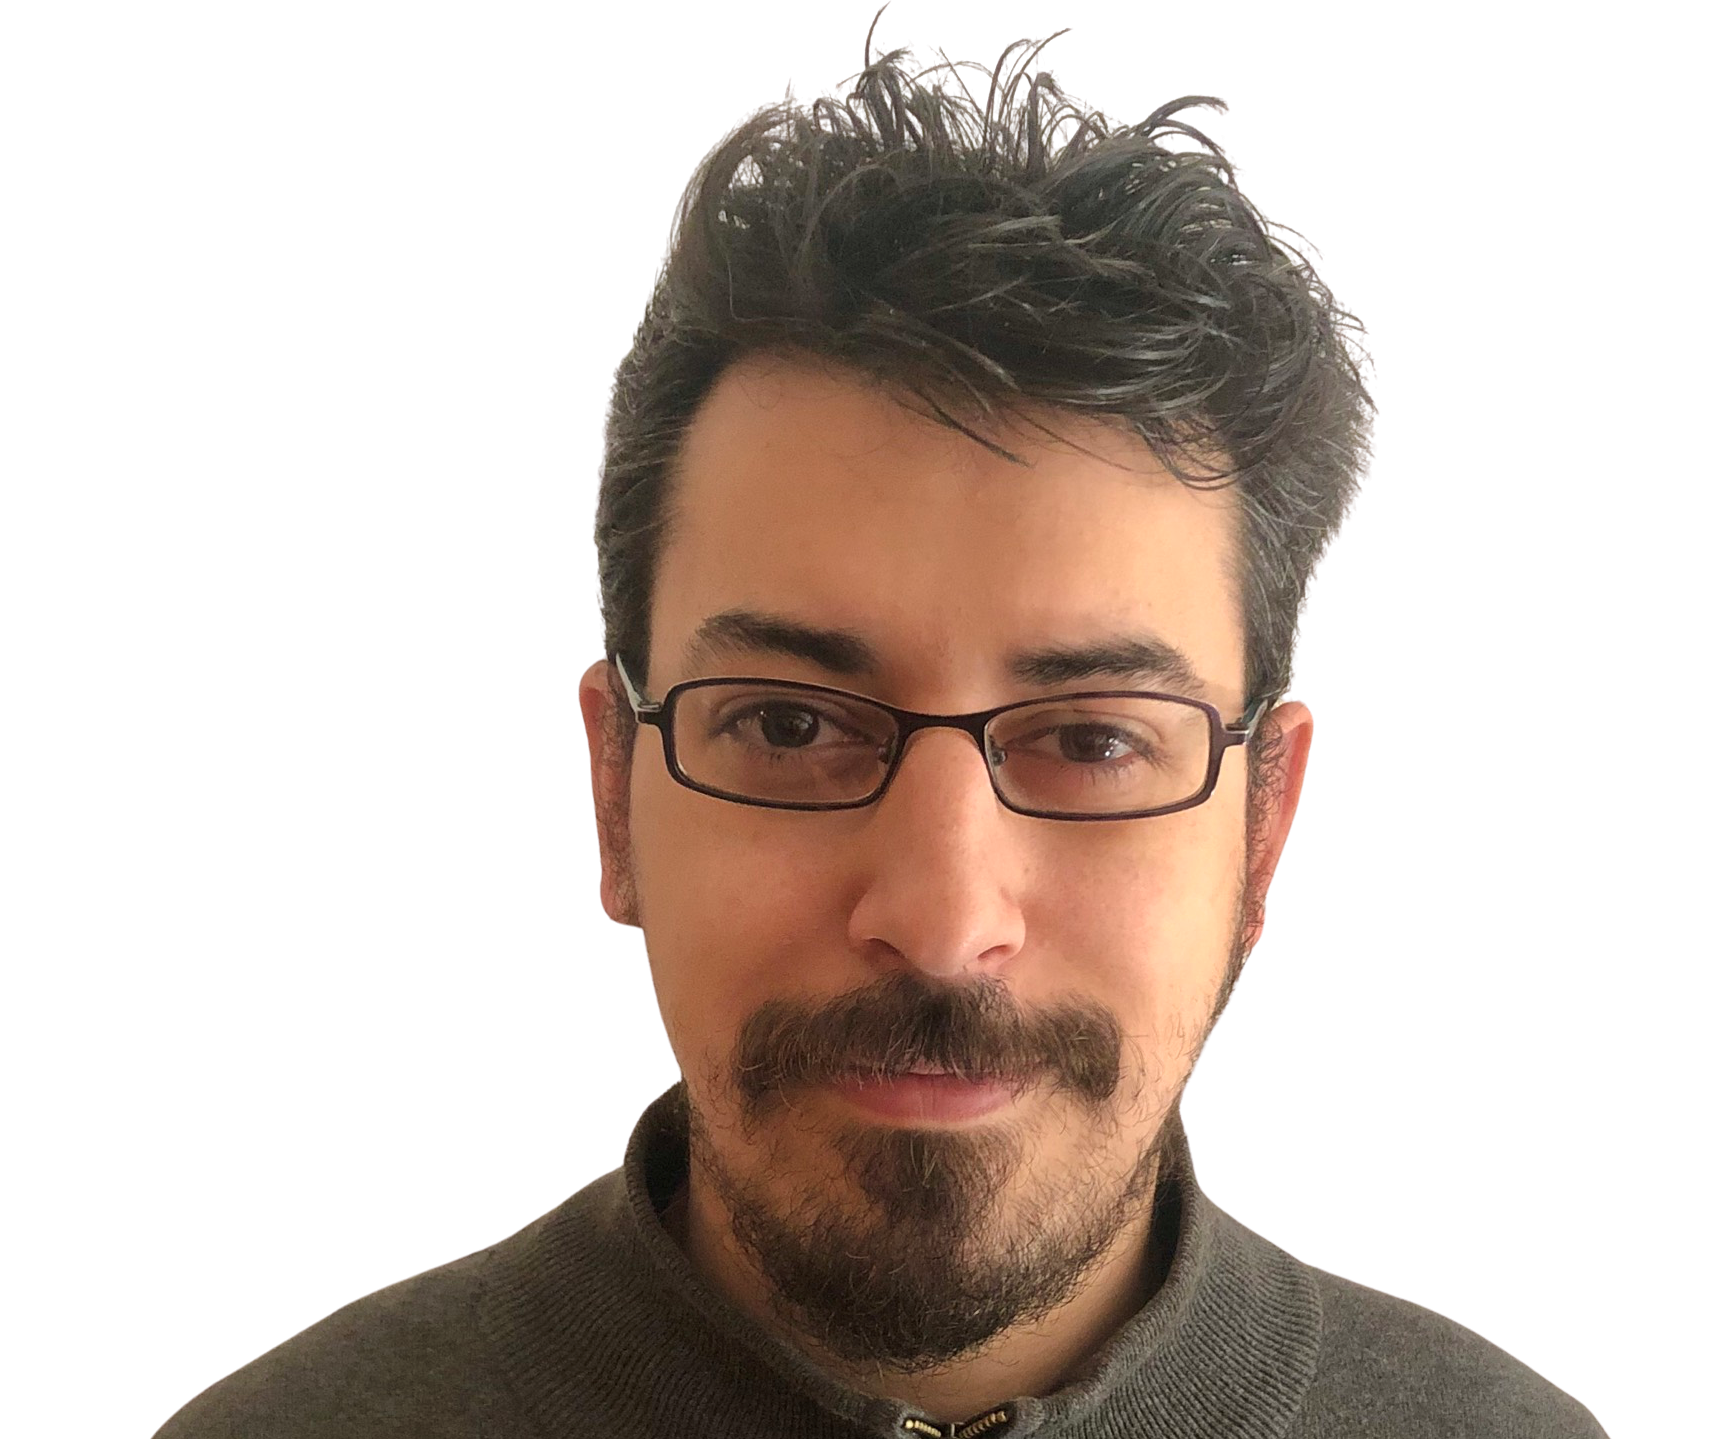
\includegraphics[width=1.05\textwidth]{images/foto_perfil.png}
				\end{figure}
			\end{column}
			\begin{column}{0.74\textwidth}
	
				\begin{itemize}
					\item Licenciado en \textbf{Matemáticas} (UGR 2009-2014).
					\item Diploma de Especialización en \textbf{Epidemiología e Investigación Clínica} (UGR, EASP, 2016).
					\item Máster de \textbf{Matemáticas} (UAL, UCA, UGR, UMA, UJA, 2019).
					\item Máster en \textbf{Ciencia de Datos }e Ingeniería de Computadores (UGR, 2020).
					\item Doctorando en Medicina Clínica y Salud Pública. Línea de investigación de Epidemiología y Salud Pública.
					\item Técnico de investigación de un proyecto de la \textbf{Asociación Española Contra el Cáncer}.
				\end{itemize}
	
			\end{column}
		\end{columns}
	\end{block}
\end{frame}

%--------------------------------------------------

\begin{frame}\frametitle{}
	\Large{\textbf{Índice}}\\[2ex]
	\normalsize
	\begin{enumerate}
		\item Epidemiología y cáncer\\[2ex]
		\item Herramientas\\[2ex]
		\item Series temporales \\[2ex]
		\item Machine learning  \\[2ex]
		\item Análisis espacial \\[2ex]
	\end{enumerate}
\end{frame}

%--------------------------------------------------

\begin{frame}\frametitle{}	
	\Large{\textbf{Índice}}\\[2ex]
	\normalsize
	\begin{enumerate}
		\item \textbf{Epidemiología y cáncer}\\[2ex]
		\item Herramientas\\[2ex]
		\item Series temporales \\[2ex]
		\item Machine learning  \\[2ex]
		\item Análisis espacial \\[2ex]
	\end{enumerate}
\end{frame}

%--------------------------------------------------

\begin{frame}\frametitle{Epidemiología y cáncer}
	\begin{block}{Epidemiología}
		La epidemiología es la ciencia que estudia la frecuencia y distribución de las enfermedades en las poblaciones humanas, así como las causas que los producen.
	\end{block}

	\begin{block}{Cáncer}
		El cáncer es una enfermedad en la que se produce una división incontrolada de las células. No es una única enfermedad, sino un conjunto de enfermedades (+100 tipos distintos de cáncer).
	\end{block}
\end{frame}

%--------------------------------------------------

%\begin{frame}\frametitle{Epidemiología y cáncer}
%	\begin{block}{Indicadores epidemiológicos}
%		Para medir el impacto del cáncer en una población se utilizan los siguientes indicadores:\\
%		\begin{enumerate}
%			\item \textbf{Incidencia}. Casos nuevos de cáncer. Mide el riesgo de presentar cáncer.\\[2ex]
%			\item \textbf{Mortalidad}. Defunciones por cáncer. Mide el riesgo de morir por cáncer.\\[2ex]
%			\item \textbf{Prevalencia}. Casos de cáncer. Mide la carga asistencial de la enfermedad.\\[2ex]
%			\item \textbf{Supervivencia}. Tiempo de supervivencia de los pacientes. Mide la historia natural de la enfermedad y efectividad del tratamiento. \\[2ex]
%		\end{enumerate}
%	\end{block}
%\end{frame}

%--------------------------------------------------


\begin{frame}\frametitle{Epidemiología y cáncer}
	\begin{block}{¿Por qué es importante investigar en cáncer?}
		\begin{enumerate}
			\item Es una enfermedad \textbf{muy frecuente}: 19 millones de casos anuales en todo el mundo, 282.000 en España.\\ \Large{\textbf{1 de cada 3 mujeres} y \textbf{1 de cada 2 hombres} desarrollará cáncer a lo largo de su vida.}\\[2ex]
			\item \normalsize Es una enfermedad con \textbf{alta mortalidad}: 10 millones de defunciones anuales por cáncer en el mundo, 113.000 en España. La supervivencia a 5 años está en torno al 60\%, con diferencias por sexos y localizaciones.\\[2ex]
		\end{enumerate}
	\end{block}
\end{frame}

%--------------------------------------------------

\begin{frame}\frametitle{Epidemiología y cáncer}
	\begin{block}{¿Qué ciencias son útiles para investigar en cáncer?}
		\begin{itemize}
			\item Medicina
			\item Enfermería
			\item Biología
			\item Nutrición
			\item Ciencias ambientales
			\item Psicología
			\item Matemáticas
			\item \textbf{\large{Estadística}}
			\item Y muchas más...
		\end{itemize}
		Equipos \textbf{interdisciplinares}.
	\end{block}
\end{frame}

%--------------------------------------------------


\begin{frame}\frametitle{Epidemiología y cáncer}
	\begin{block}{Registro de Cáncer de Granada}
		\begin{itemize}
			\item Escuela Andaluza de Salud Pública (Campus de Cartuja).
			\item Recoge todos los casos de cáncer de la provincia de Granada desde 1985: +130.000 casos.
			\item Equipo: 14 personas (2 matemáticos, 2 bioestadísticos).
		\end{itemize}
		
	\vspace{-10pt}	
	\begin{columns}
		\begin{column}{.5\textwidth}
		\begin{figure}
			\centering
			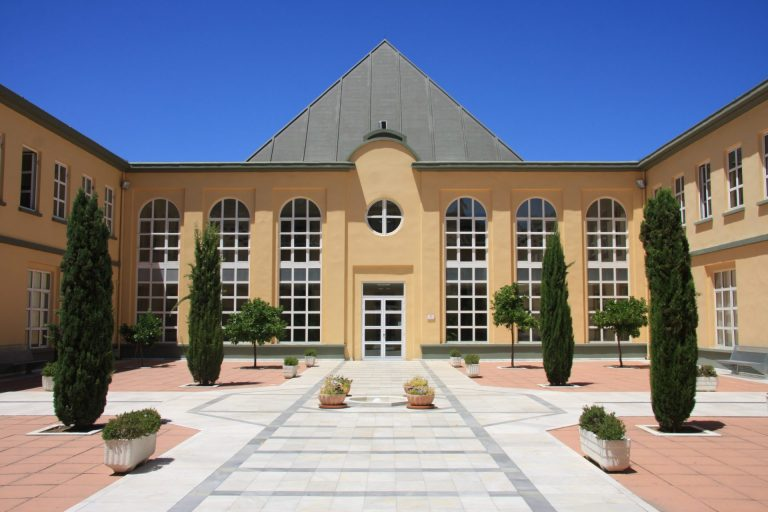
\includegraphics[width=.9\textwidth]{images/registro.jpg}
		\end{figure}
		\end{column}
		\begin{column}{.5\textwidth}
			\begin{figure}
				\centering
			\includegraphics[width=.9\textwidth]{logos/logo_rcg.png}
			\end{figure}
		\end{column}
	\end{columns}
	
	\vspace{5pt}
	\centering
	\textit{\url{www.registrocancergranada.es}}
	\end{block}
\end{frame}

%--------------------------------------------------

\begin{frame}\frametitle{Epidemiología y cáncer}
	\begin{block}{Algunas tareas de un estadístico en un Registro de Cáncer}
		\begin{itemize}
			\item Mantenimiento de base de datos.
			\item Control de calidad.
			\item Cálculo de tasas: brutas, estandarizadas, acumulativas, truncadas.
			\item Generación de tablas estadísticas.
			\item Automatización de procesos.
			\item Diseño epidemiológico.
			\item Elaboración de informes y artículos científicos.
			\item Divulgación científica.
		\end{itemize}
	\end{block}	
\end{frame}


%--------------------------------------------------
\begin{frame}\frametitle{}
	\Large{\textbf{Índice}}\\[2ex]
	\normalsize
	\begin{enumerate}
		\item Epidemiología y cáncer\\[2ex]
		\item \textbf{Herramientas}\\[2ex]
		\item Series temporales \\[2ex]
		\item Machine learning  \\[2ex]
		\item Análisis espacial \\[2ex]
	\end{enumerate}	
\end{frame}

%--------------------------------------------------

\begin{frame}\frametitle{Herramientas}
		\begin{columns}
			\begin{column}{0.5\textwidth}
				\begin{figure}
					\centering
					
\includegraphics[width=.7\textwidth]{images/access.png}
				\end{figure}
			\end{column}
		\huge{\textbf{+}}
			\begin{column}{0.5\textwidth}
				\centering
				\begin{figure}
					\centering
					
\includegraphics[width=.8\textwidth]{images/vba.png}
				\end{figure}
				\begin{figure}
					\centering
					
\includegraphics[width=.5\textwidth]{images/sql.png}
				\end{figure}
			\end{column}
		\end{columns}
\end{frame}

%--------------------------------------------------

\begin{frame}\frametitle{Herramientas}	
	\begin{columns}
		\begin{column}{0.5\textwidth}
			\begin{figure}
				\centering
				
\includegraphics[width=.5\textwidth]{logos/logo_R.png}
			\end{figure}
			\begin{figure}
				\centering
				
\includegraphics[width=.7\textwidth]{images/rstudio.png}
			\end{figure}
		\end{column}
		\huge{\textbf{+}}
		\begin{column}{0.5\textwidth}
			\centering
			\begin{figure}
				\centering
				\includegraphics[width=.95\textwidth]{images/R_paquetes.png}
			\end{figure}
		\end{column}
	\end{columns}
\end{frame}

%--------------------------------------------------

\begin{frame}\frametitle{Herramientas}
	\begin{columns}
		\begin{column}{0.4\textwidth}
			\begin{figure}
				\centering
				
\includegraphics[width=.7\textwidth]{images/stata.jpg}
			\end{figure}
		
			\vspace{50pt}
			
			\centering
			\textbf{Trabajo en equipo}
			
		\end{column}
		\begin{column}{0.6\textwidth}
			\centering
			Software específico de Registros de Cáncer:\\

			\begin{itemize}
				\item 			\centering Control de calidad
				\item 			\centering Conversión de codificaciones
				\item 			\centering Análisis de tendencias
			\end{itemize}	
			\vspace{41pt}
			\centering
			\textbf{Inglés}
		\end{column}
	\end{columns}
	
	\vspace{25pt}
	\centering
	\textbf{Estadística pública}: poblaciones, defunciones, censos, encuestas...
\end{frame}

%--------------------------------------------------

\begin{frame}\frametitle{Herramientas}
	\begin{block}{Visualización de datos}
		\begin{itemize}
			\item Un gráfico vale más que mil palabras.
			\item Deben ser \textbf{claros} y \textbf{precisos}.
			\item Hay que saber \textbf{interpretar} y \textbf{crear} gráficos.
			\item A veces son convenientes \textbf{gráficos interactivos}: \url{https://www.danielredondo.com/grafico2}
			\item Es uno de los puntos fuertes de R con el paquete  \{ggplot2\}.
		\end{itemize}
		\begin{figure}
			\centering
			
\includegraphics[width=.20\textwidth]{images/ggplot2.png}
		\end{figure}
	\end{block}
\end{frame}

%--------------------------------------------------

\begin{frame}\frametitle{Herramientas}
	\vspace{-5pt}
	\begin{figure}
		\centering
		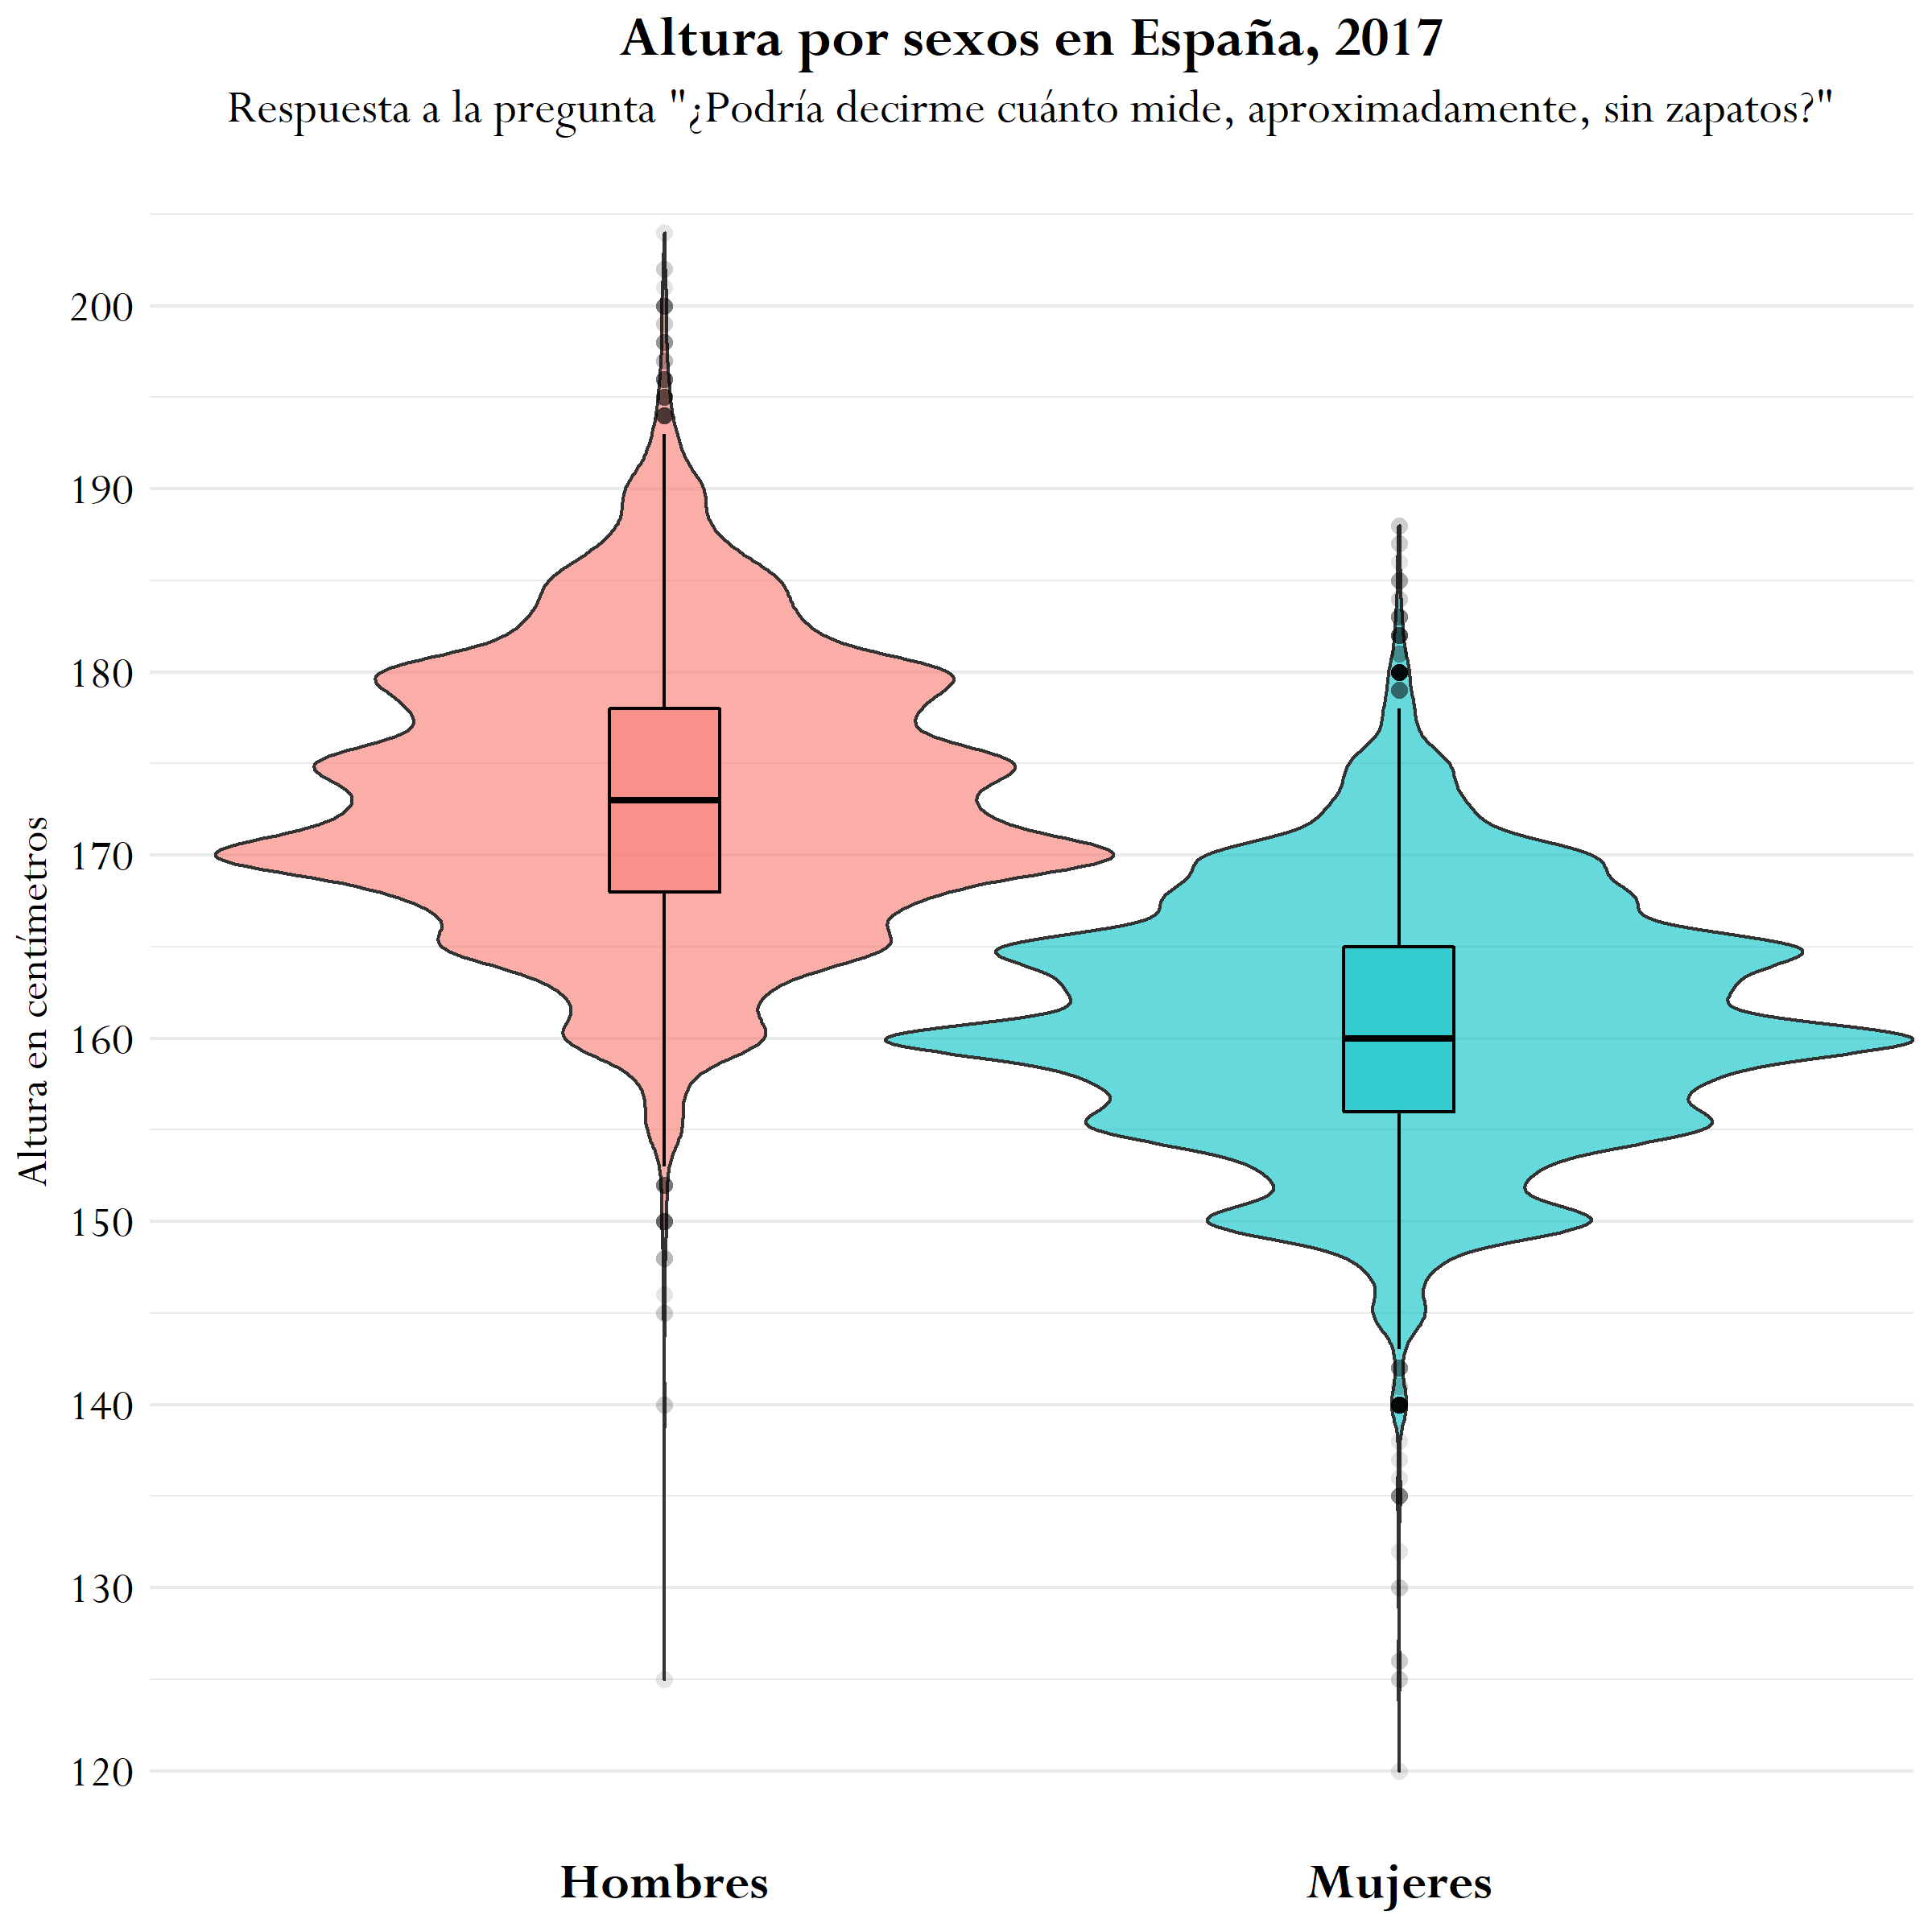
\includegraphics[width=.68\textwidth]{images/25.png}
	\end{figure}
\end{frame}

%--------------------------------------------------

\begin{frame}\frametitle{Herramientas}
	\vspace{-5pt}
	\begin{figure}
		\centering
		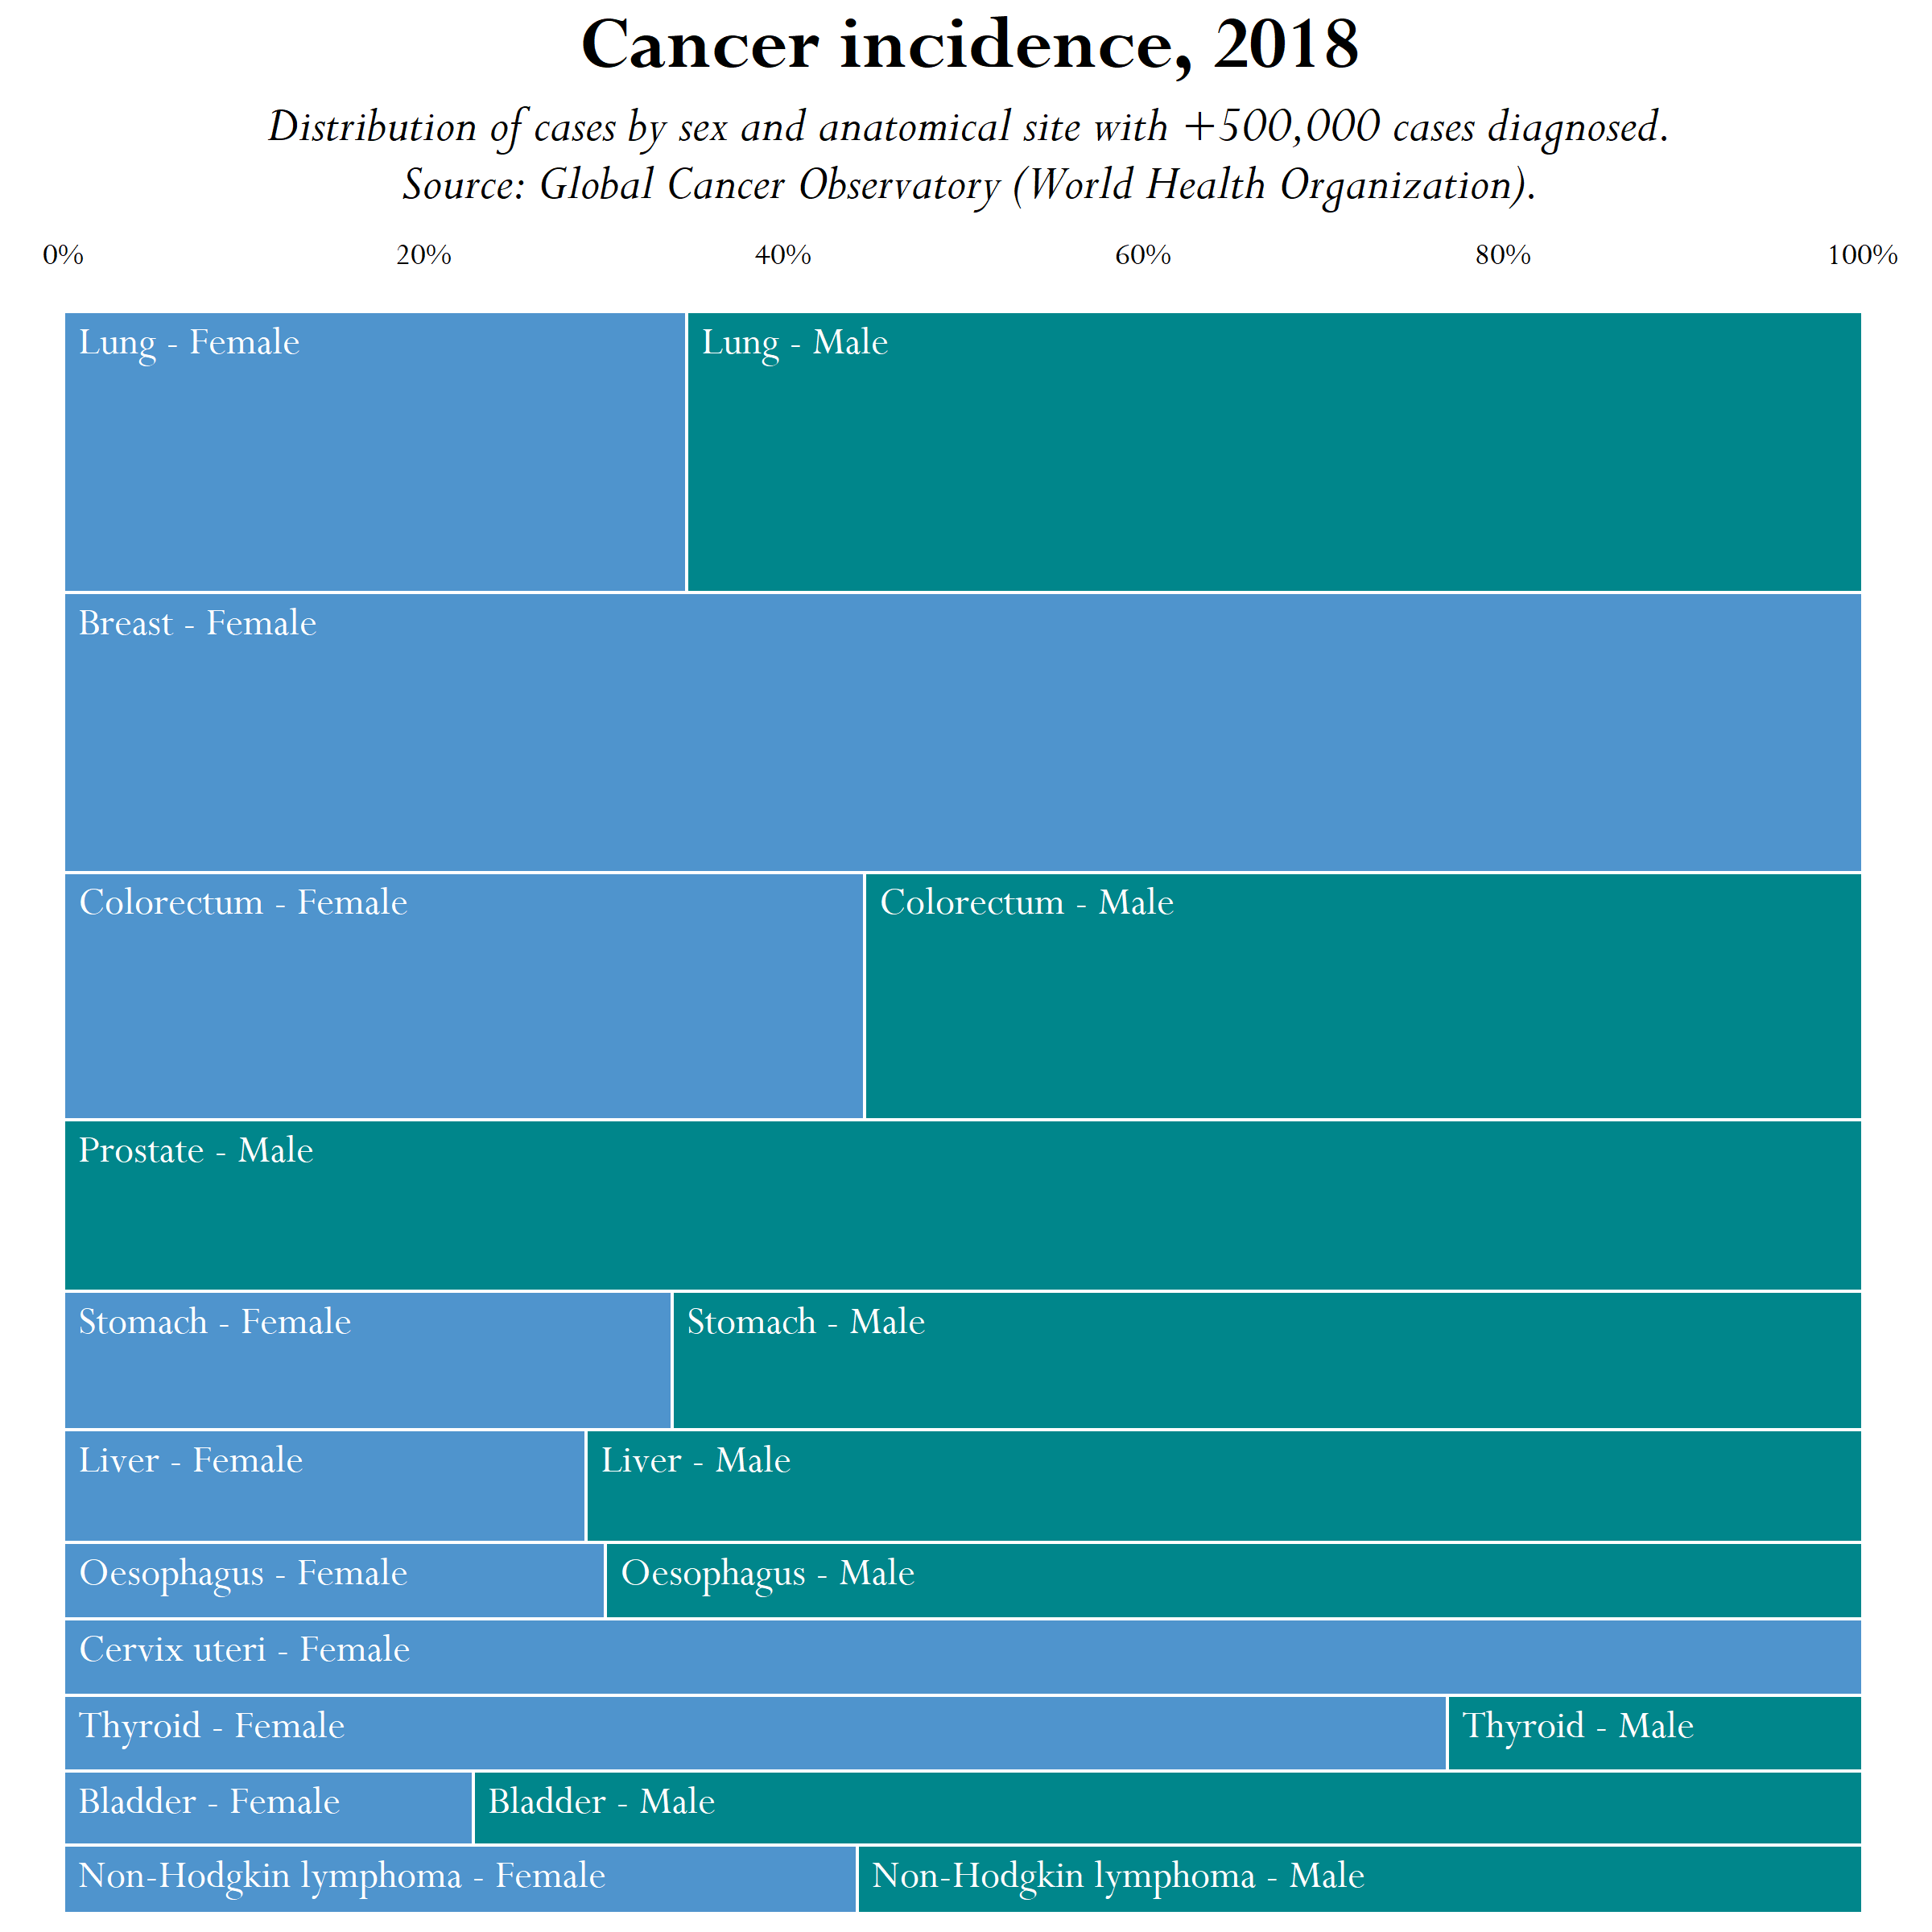
\includegraphics[width=.68\textwidth]{images/26.png}
	\end{figure}	
\end{frame}

%--------------------------------------------------

\begin{frame}\frametitle{Herramientas}
	\begin{columns}
		\begin{column}{0.5\textwidth}
			\begin{figure}
				\centering
				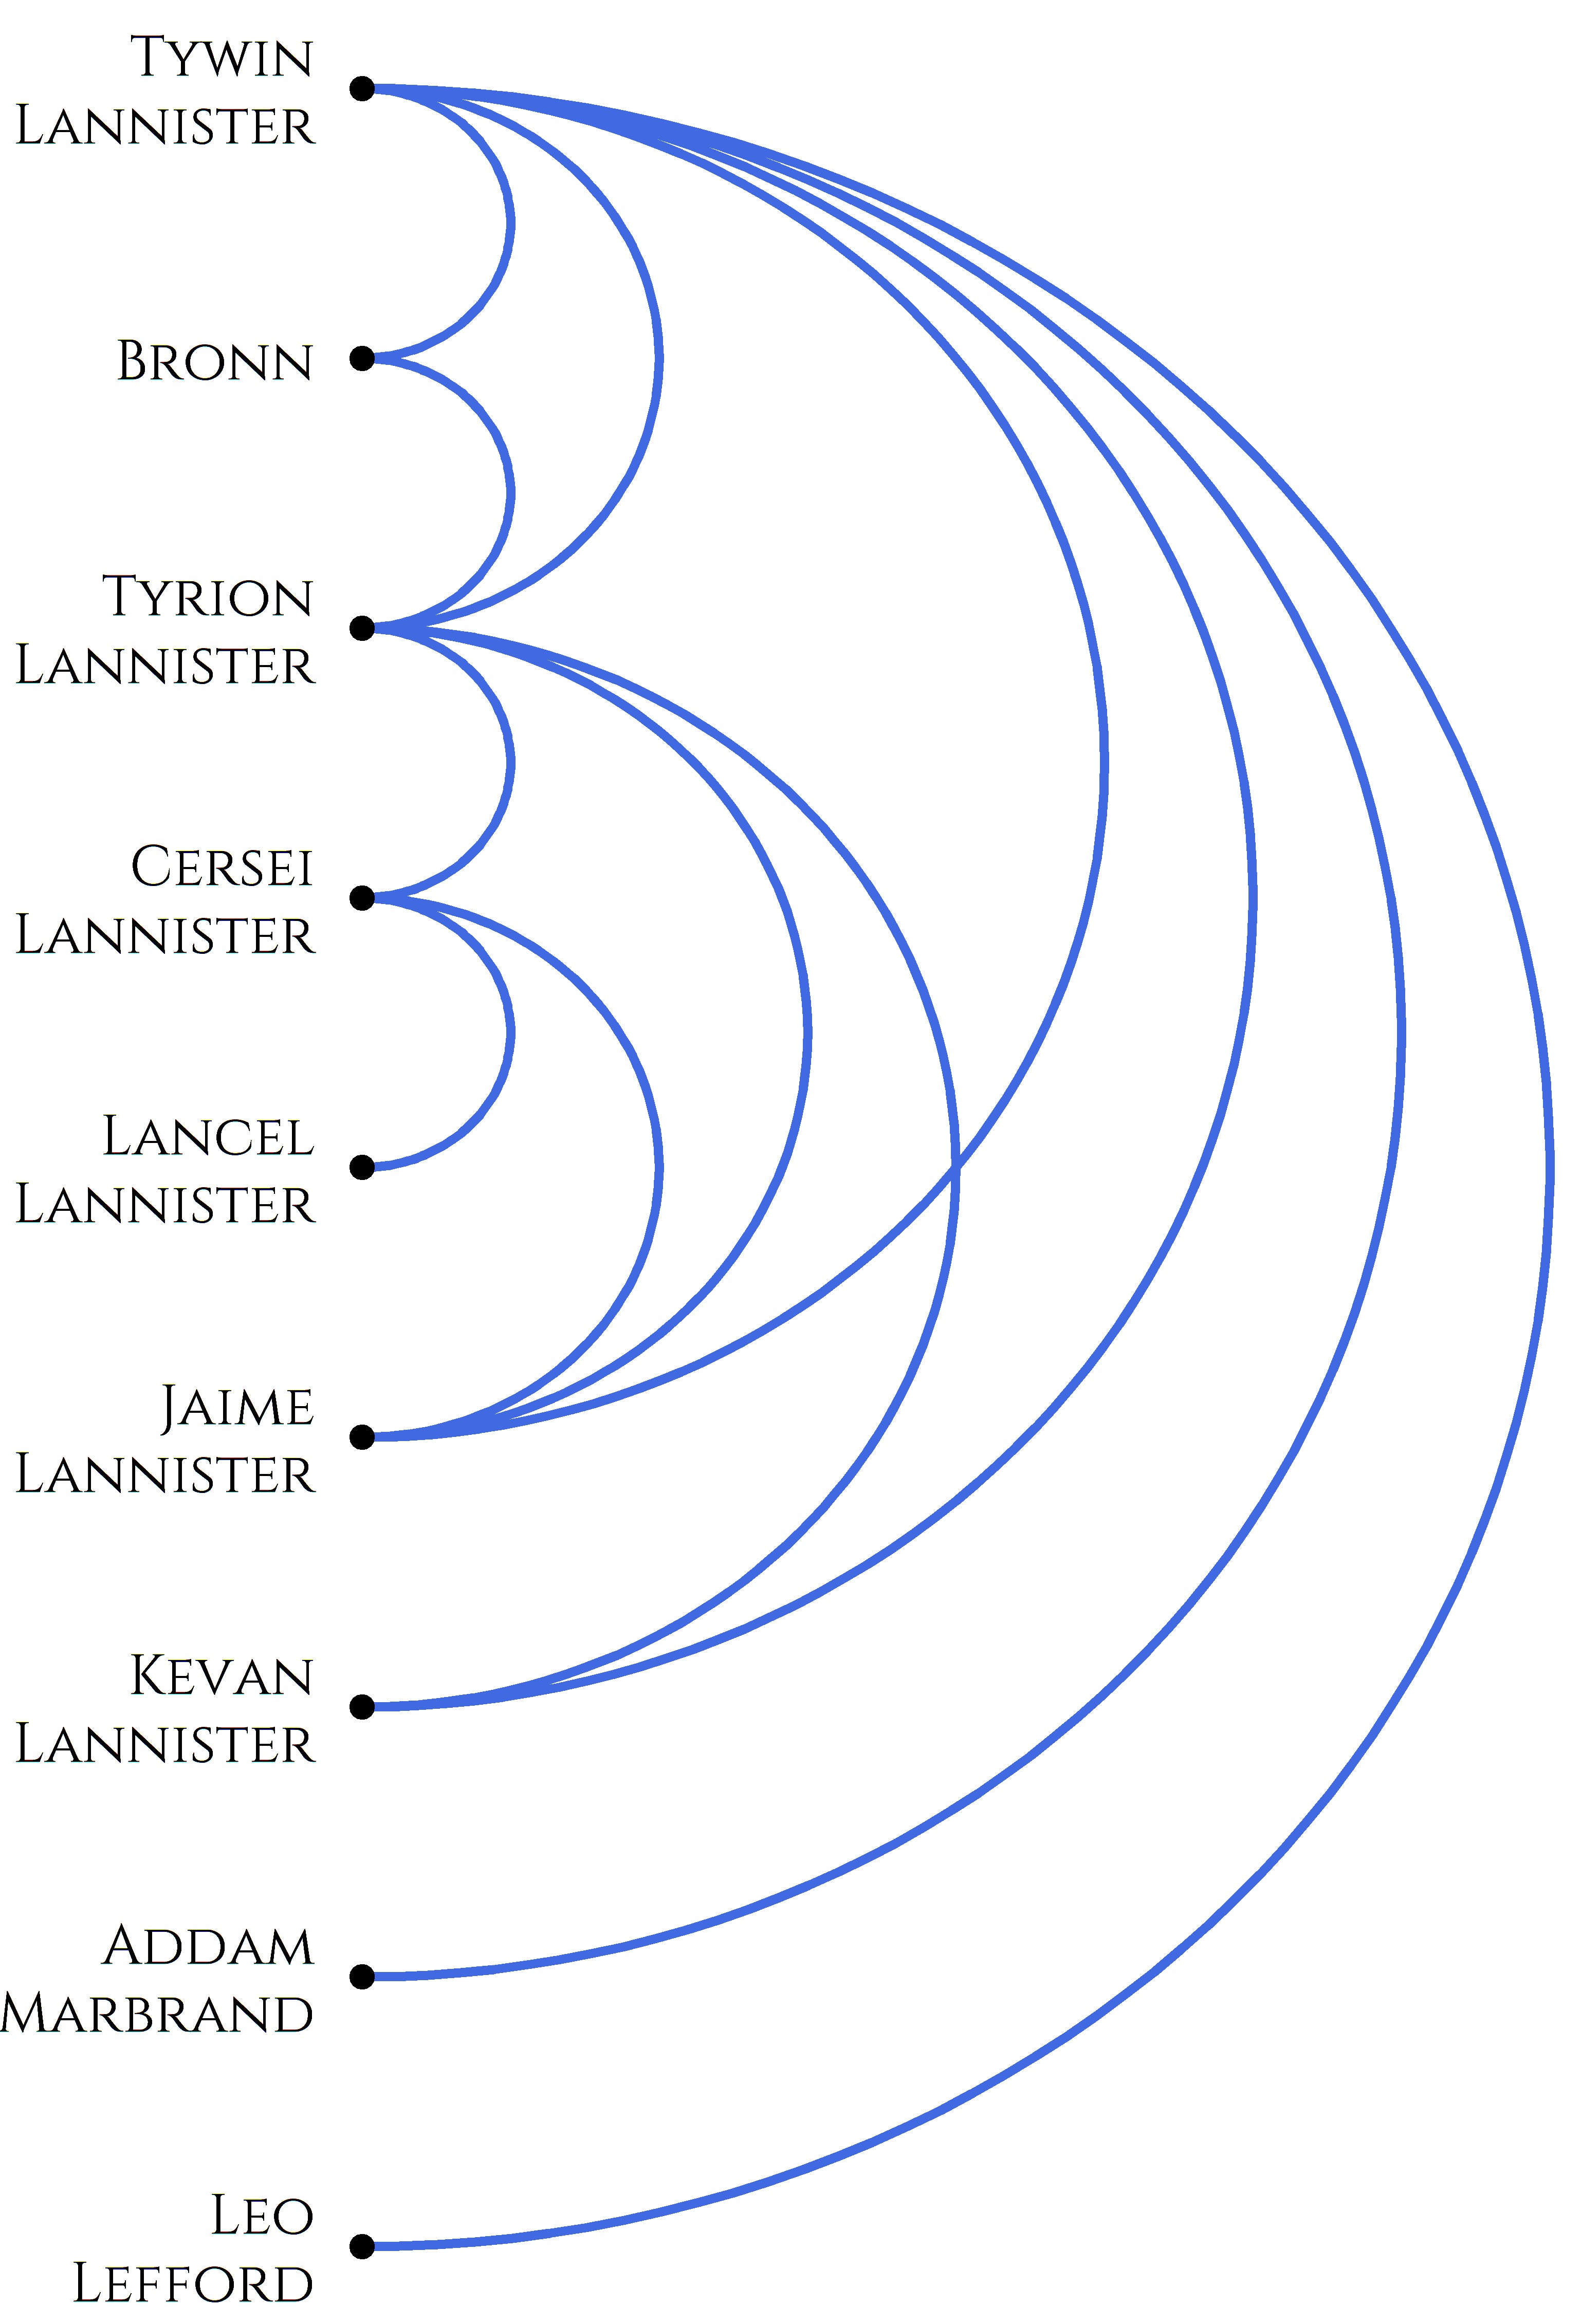
\includegraphics[width=.85\textwidth]{images/5.jpg}
			\end{figure}
		\end{column}
		\begin{column}{0.5\textwidth}
			\begin{figure}
				\centering
				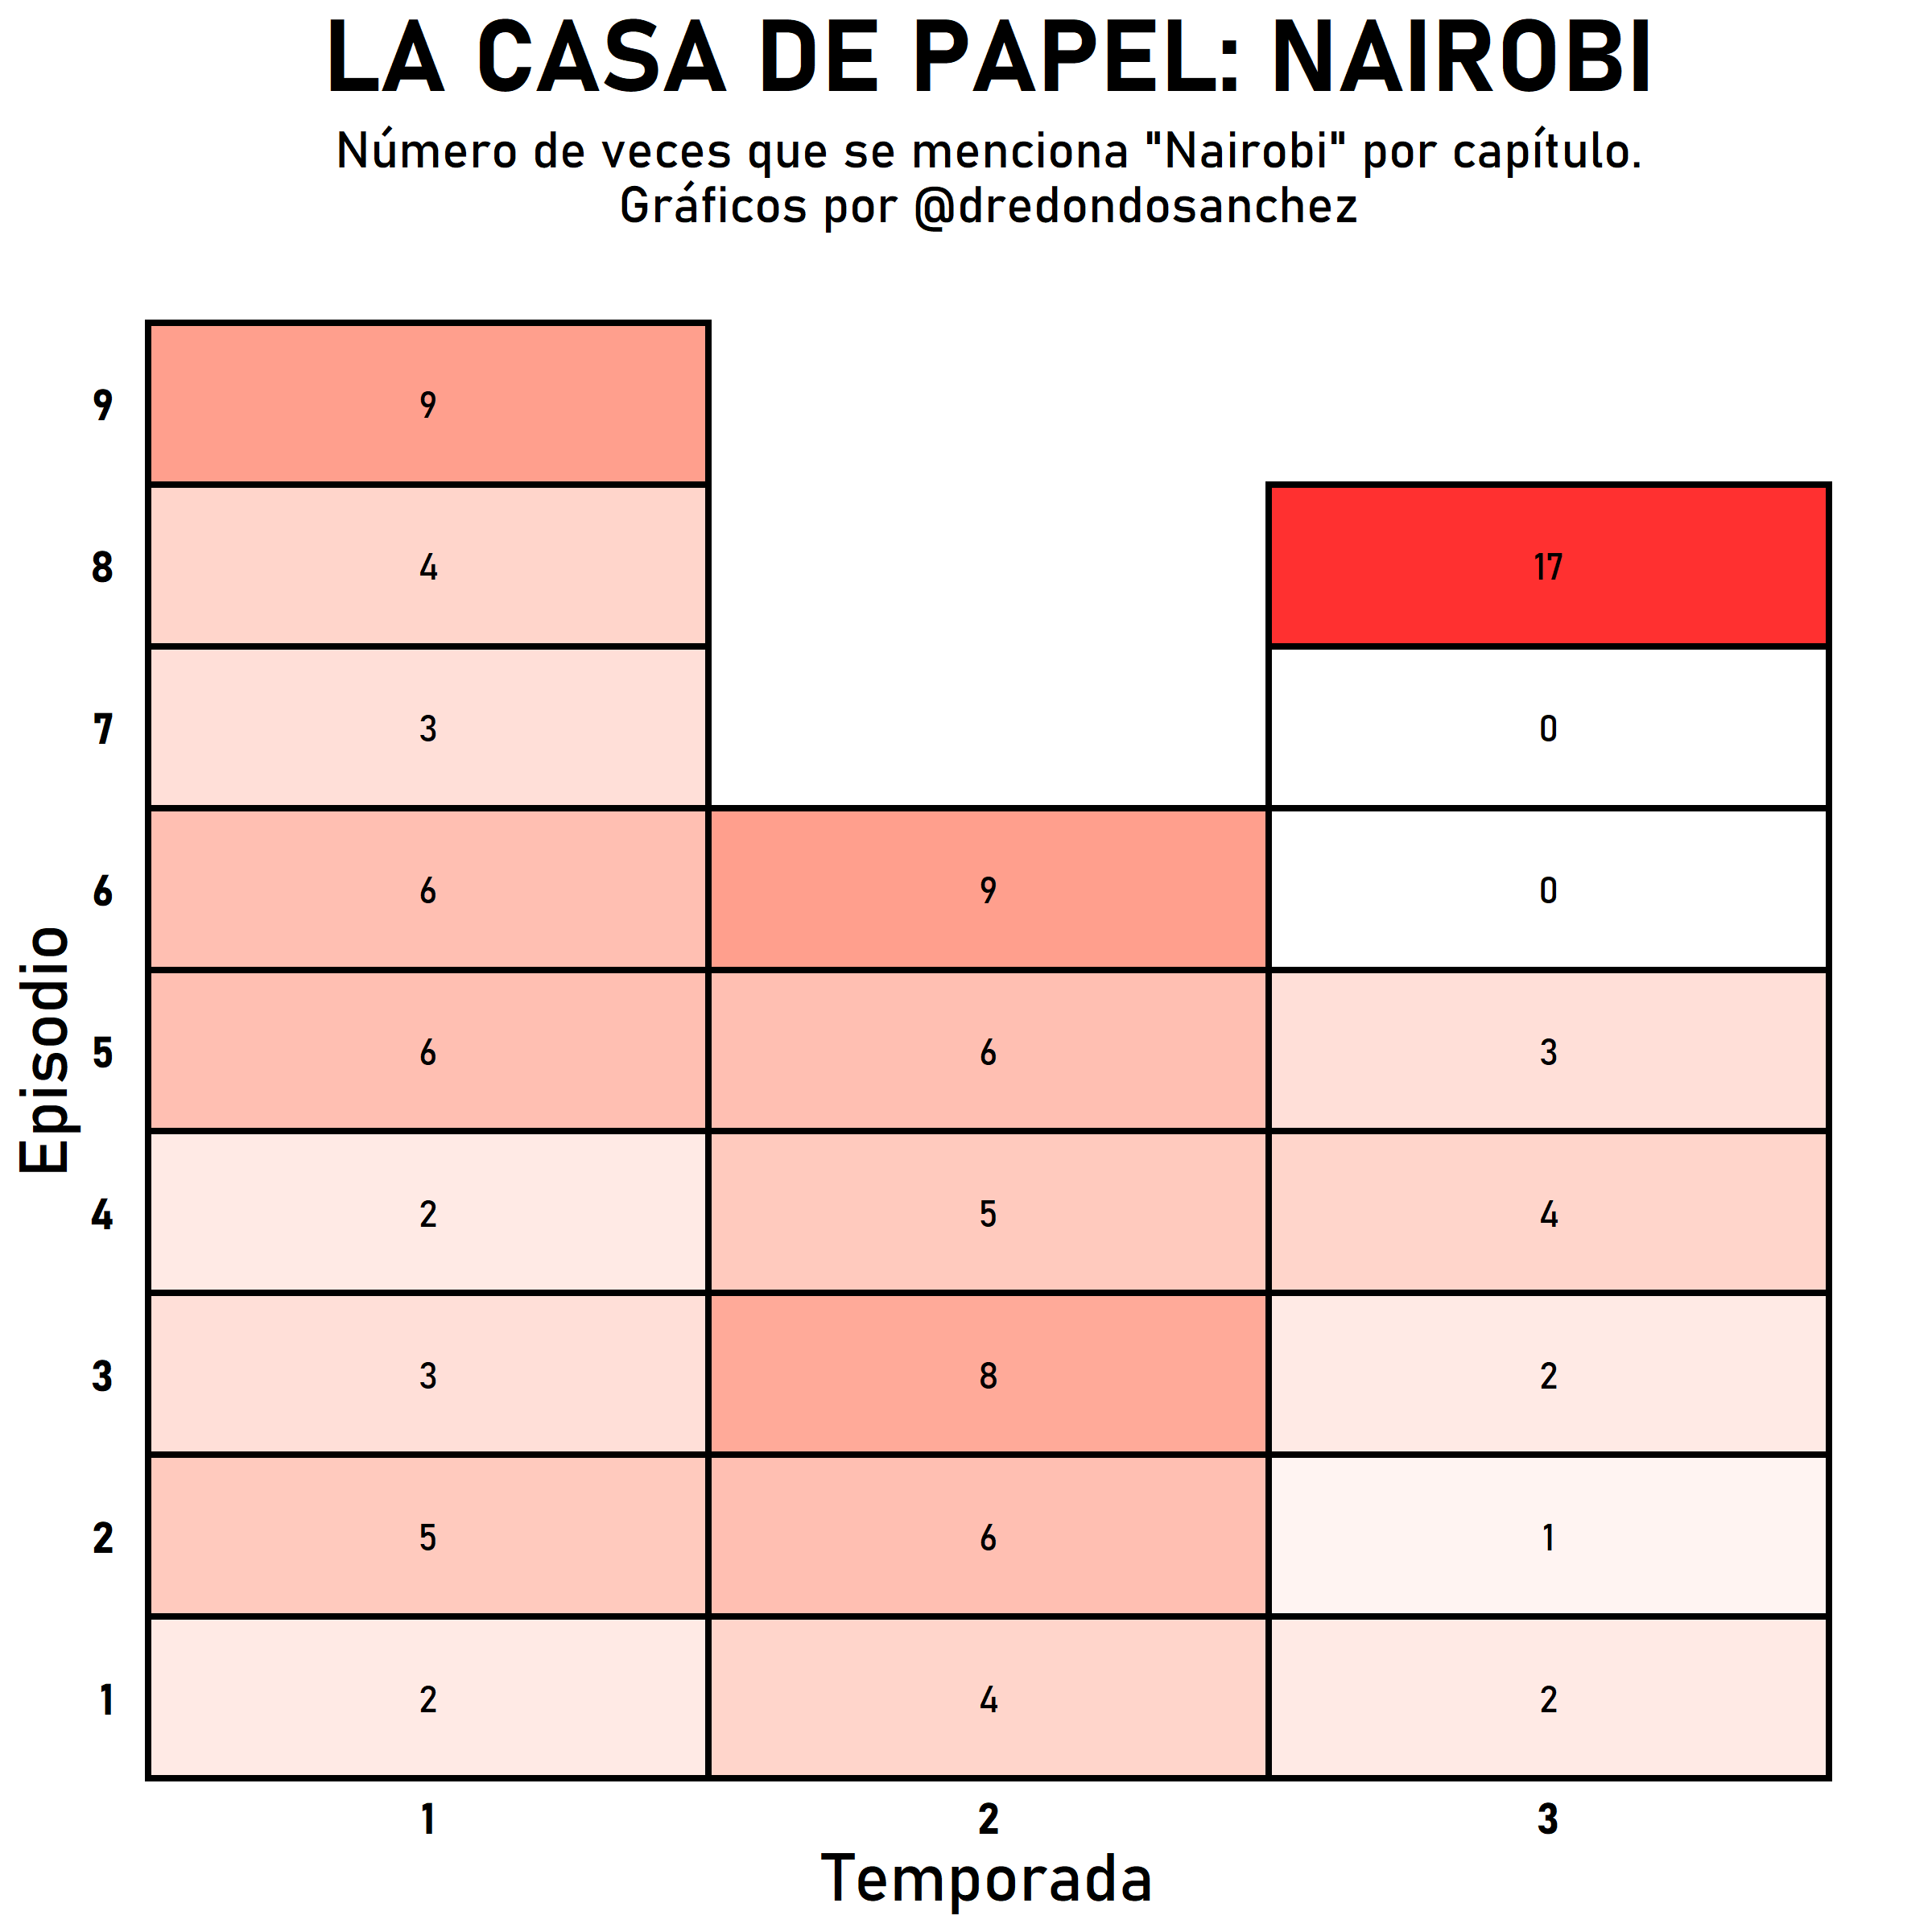
\includegraphics[width=\textwidth]{images/16.png}
			\end{figure}
		\end{column}
	\end{columns}	
\end{frame}

%--------------------------------------------------

\begin{frame}\frametitle{Herramientas}
	\begin{figure}
		\centering
		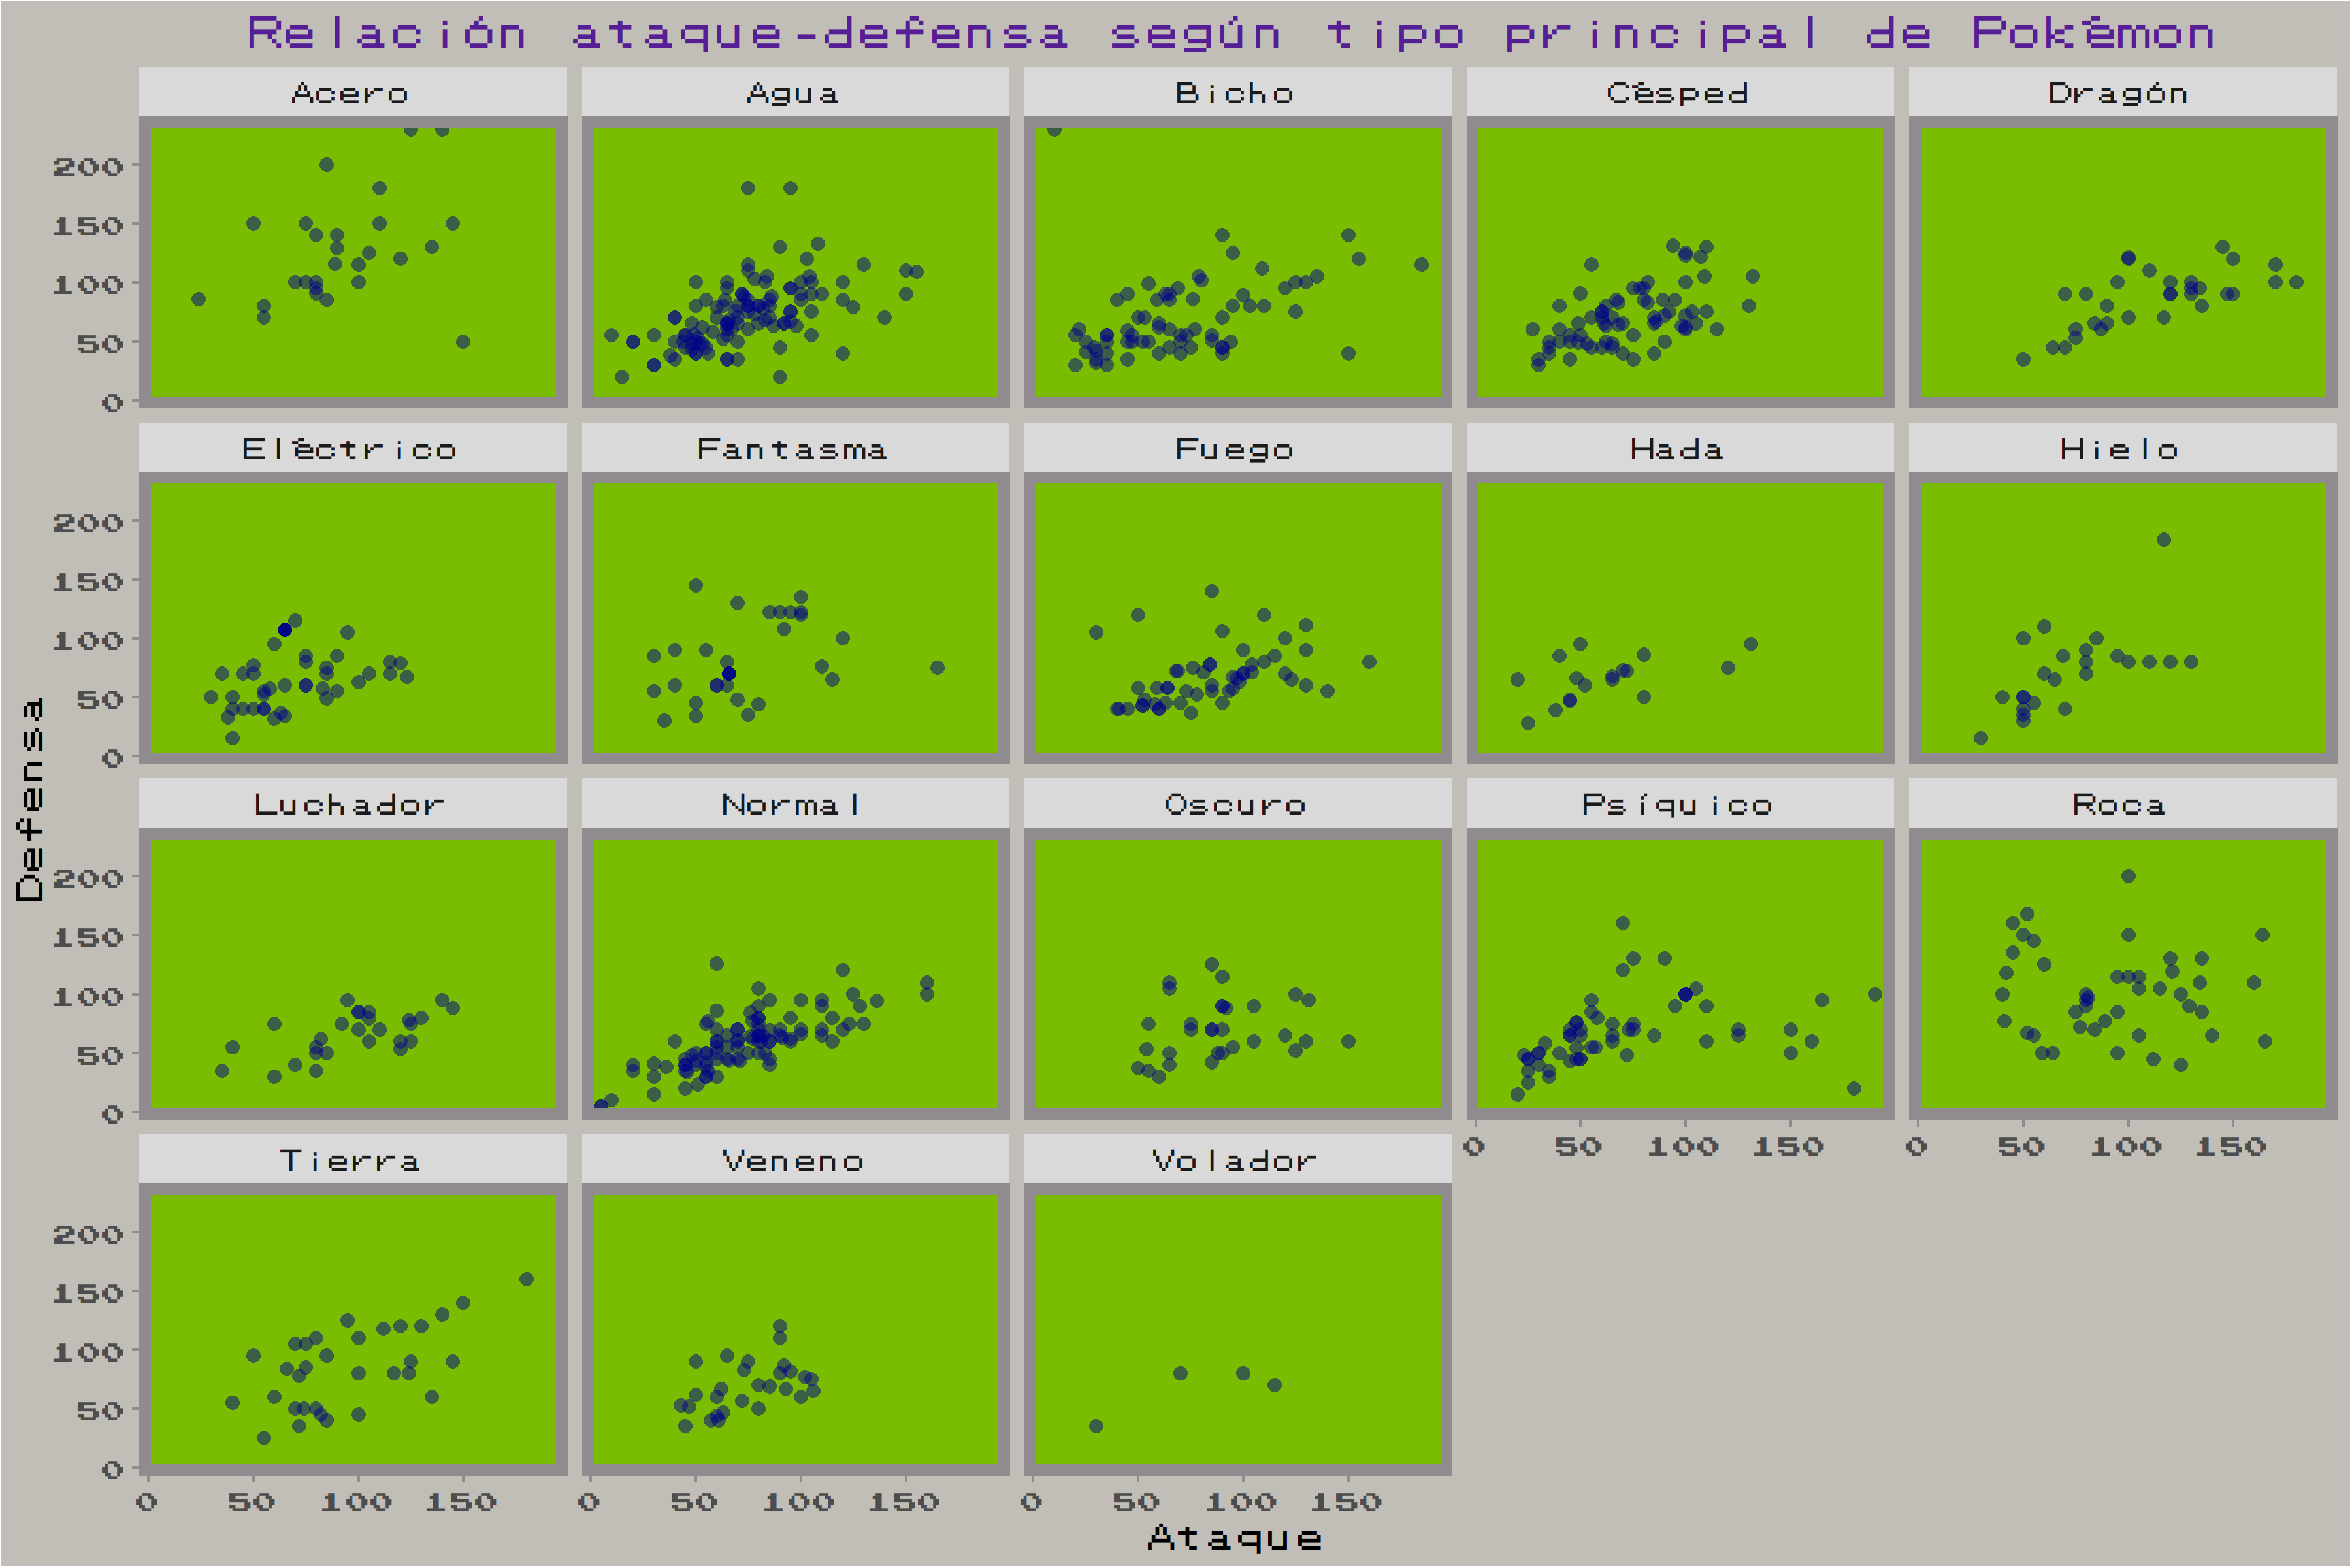
\includegraphics[width=.95\textwidth]{images/4.png}
	\end{figure}
\end{frame}

%------------------------------------------------

\begin{frame}\frametitle{}
	\Large{\textbf{Índice}}\\[2ex]
	\normalsize
	\begin{enumerate}
		\item Epidemiología y cáncer\\[2ex]
		\item Herramientas\\[2ex]
		\item \textbf{Series temporales} \\[2ex]
		\item Machine learning  \\[2ex]
		\item Análisis espacial \\[2ex]
	\end{enumerate}
\end{frame}

%--------------------------------------------------

\begin{frame}\frametitle{Series temporales}
	\begin{block}{Series temporales}
		\begin{enumerate}
			\item \textbf{Tendencias de la incidencia de cáncer}\\[2ex]
			\item Proyecciones de la incidencia de cáncer\\[2ex]
			\item Estimaciones de la incidencia de cáncer\\[2ex]
		\end{enumerate}
	\end{block}
\end{frame}

%--------------------------------------------------

\begin{frame}\frametitle{Series temporales - Tendencias}
	\centering
	Incidencia del total del cáncer. Provincia de Granada, 1985-2016.
	\begin{figure}
		\centering
		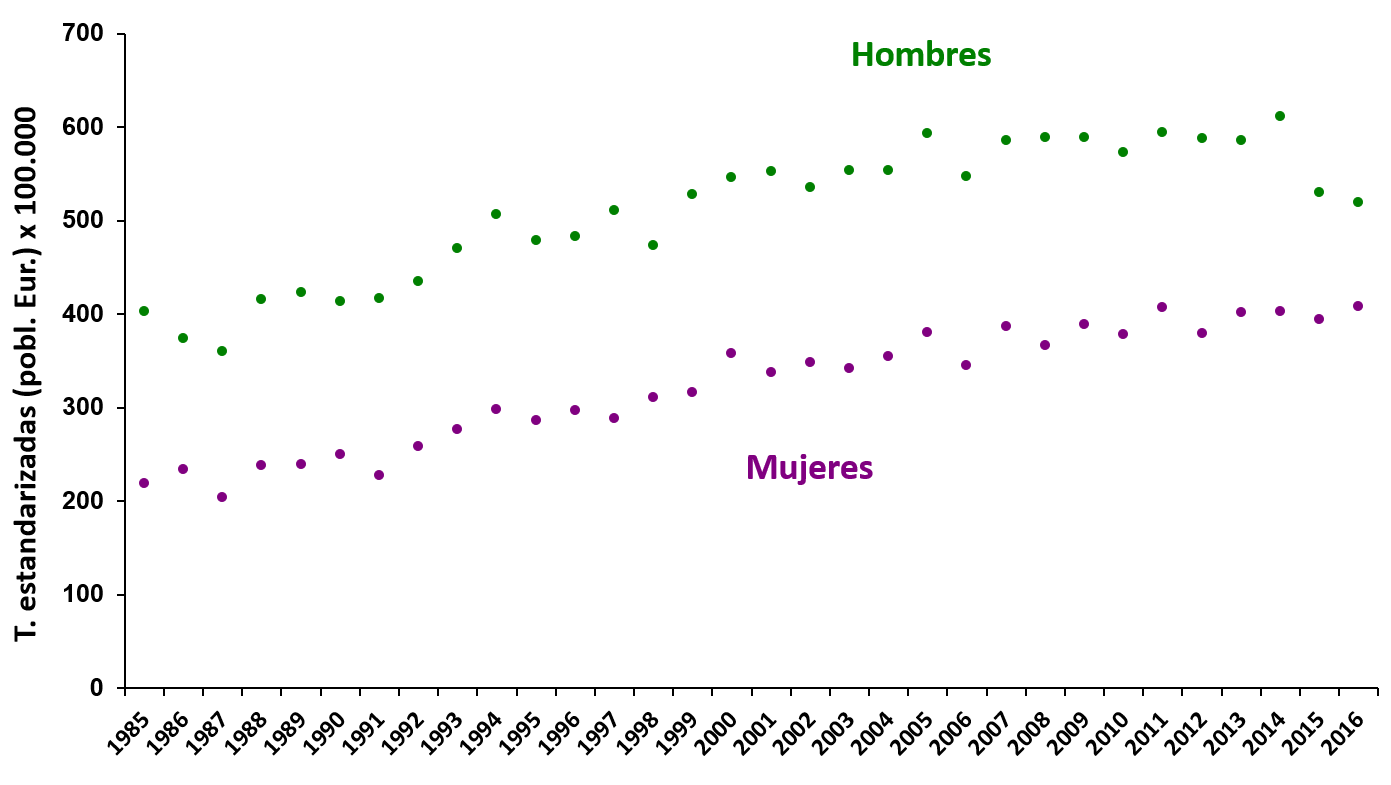
\includegraphics[width=\textwidth]{images/tendencias0.png}
	\end{figure}
\end{frame}

%--------------------------------------------------

\begin{frame}\frametitle{Series temporales - Tendencias}
	\centering
	Incidencia del total del cáncer. Provincia de Granada, 1985-2016.
	\begin{figure}
		\centering
		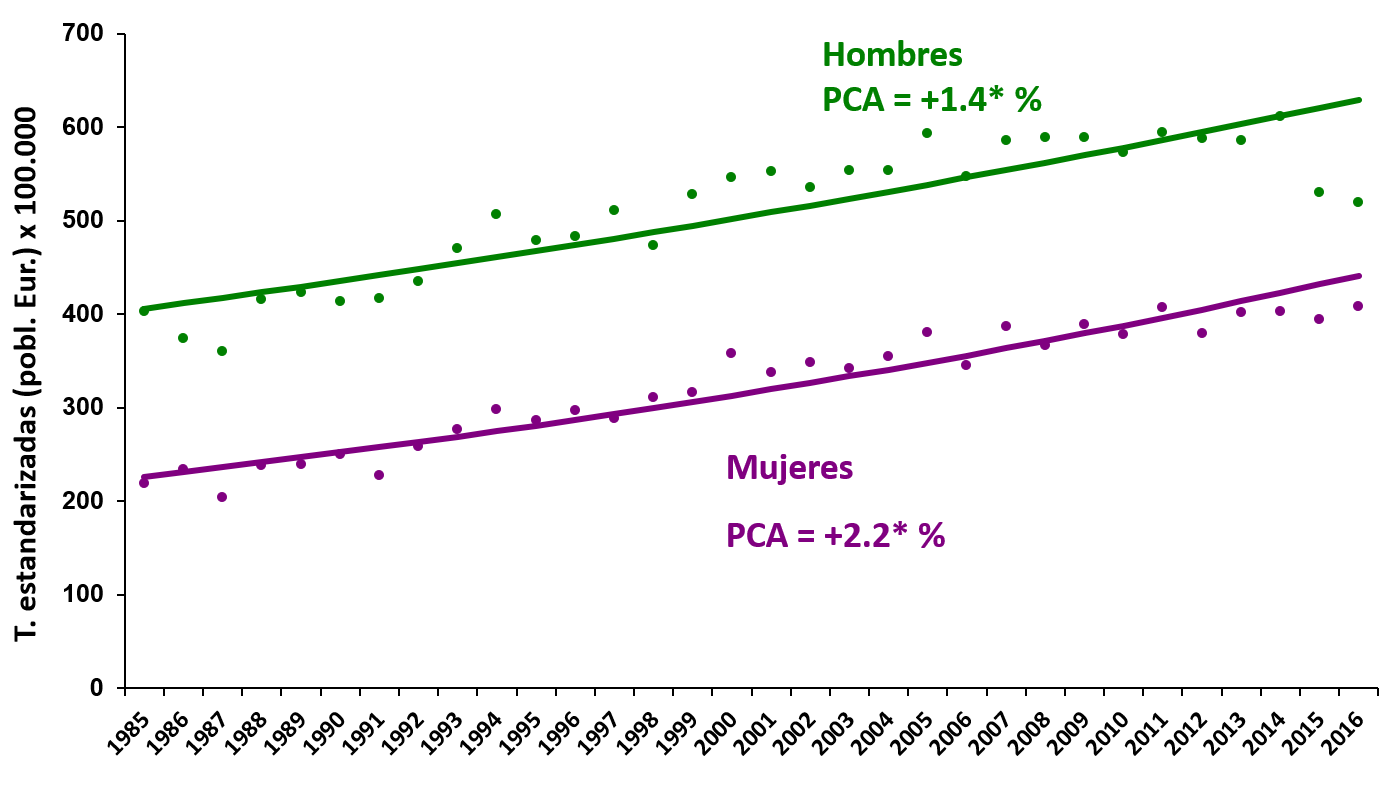
\includegraphics[width=\textwidth]{images/tendencias1.png}
	\end{figure}
\end{frame}

%--------------------------------------------------

\begin{frame}\frametitle{Series temporales - Tendencias}
	\centering
	Incidencia de cáncer de pulmón en hombres. Provincia de Granada, 1985-2016.
	\begin{figure}
		\centering
		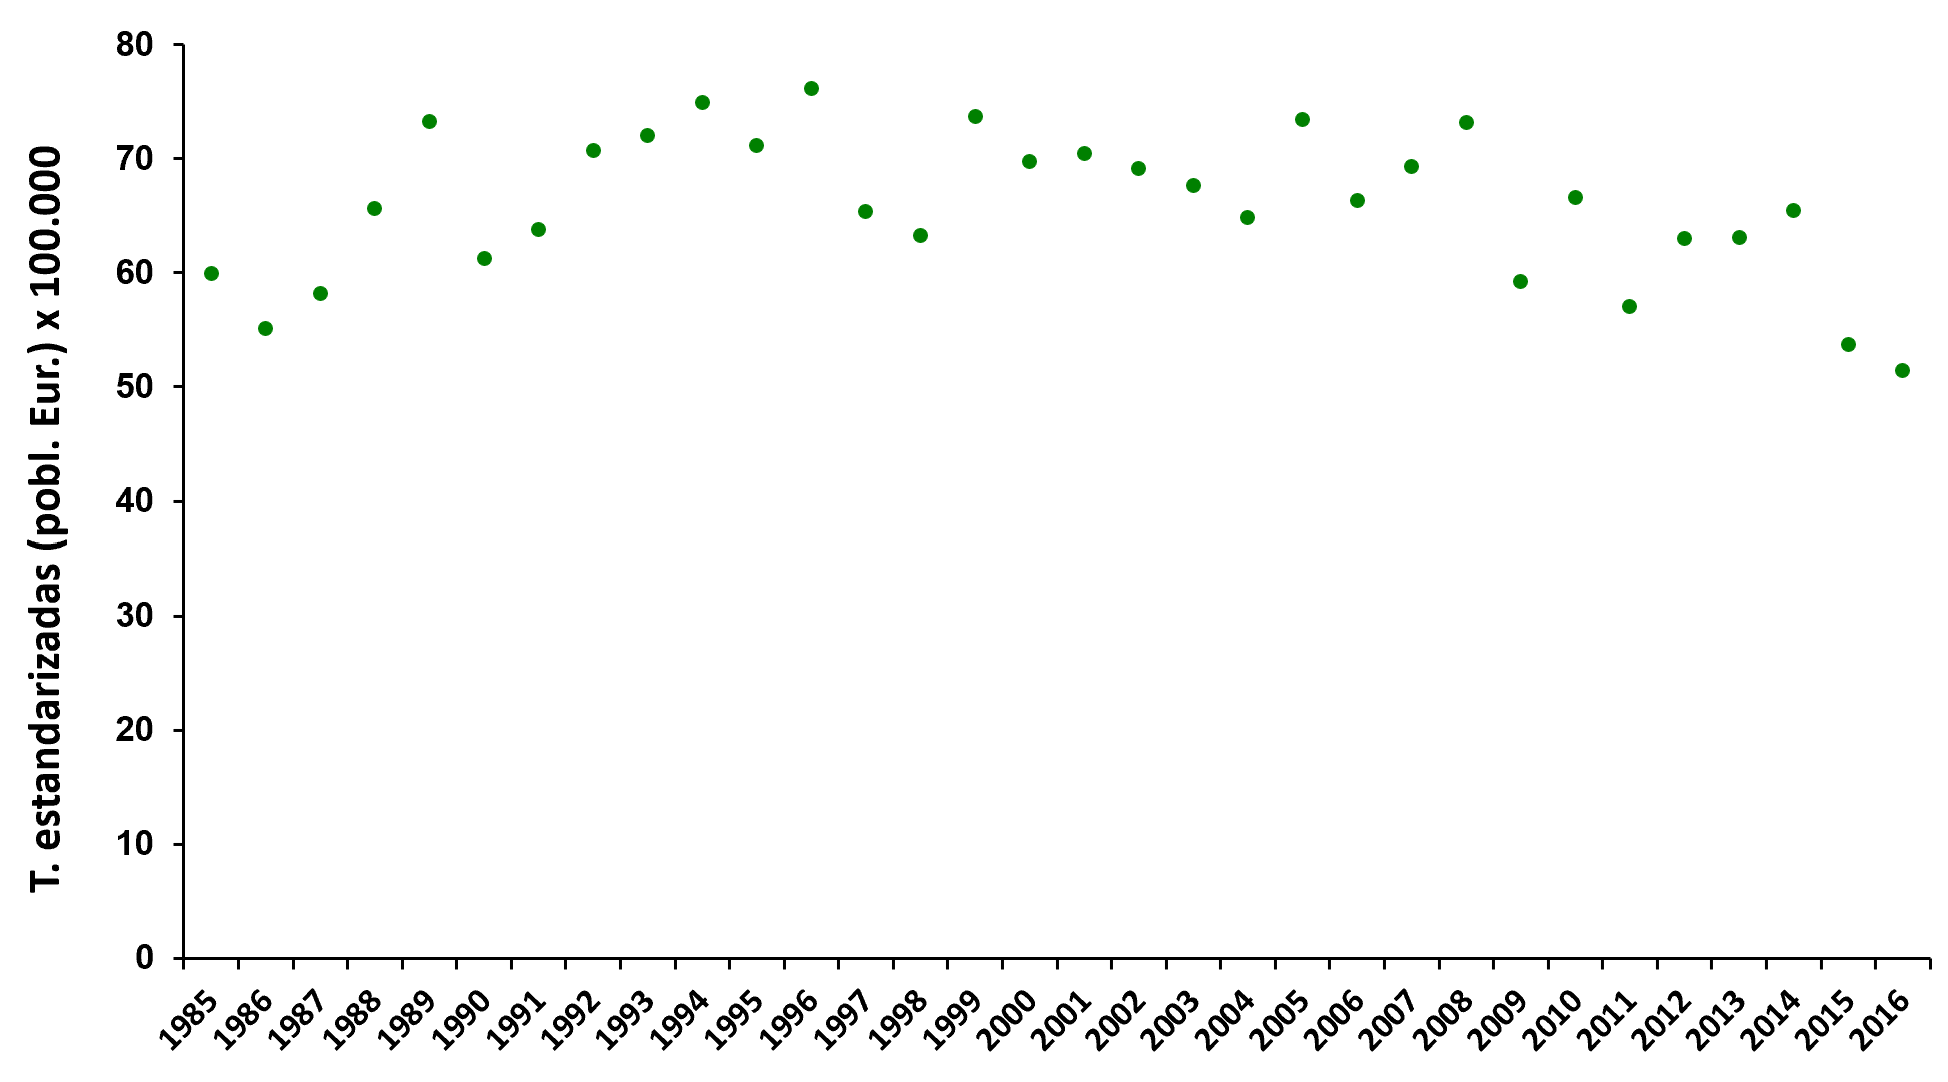
\includegraphics[width=\textwidth]{images/tendencias_pulmon0.png}
	\end{figure}
\end{frame}

%--------------------------------------------------

\begin{frame}\frametitle{Series temporales - Tendencias}
	\vspace{0pt}
	\begin{columns}
		\begin{column}{0.5\textwidth}
			\centering \normalsize 0 puntos de inflexión
			\begin{figure}
				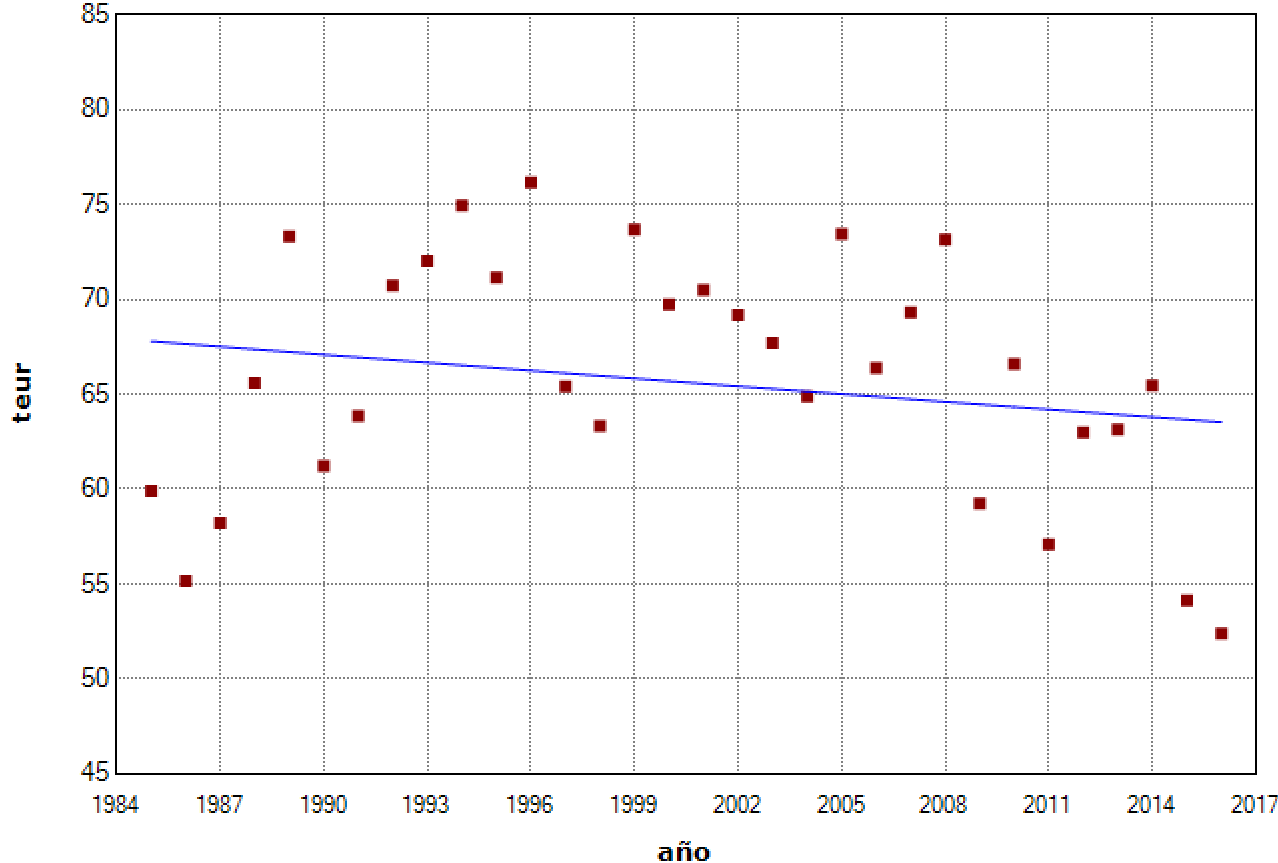
\includegraphics[width=\textwidth]{images/jpo0.png}
			\end{figure}

		\end{column}
		\large{\textbf{vs}}
		\begin{column}{0.5\textwidth}
			\centering \normalsize 5 puntos de inflexión
			\begin{figure}
				\centering
				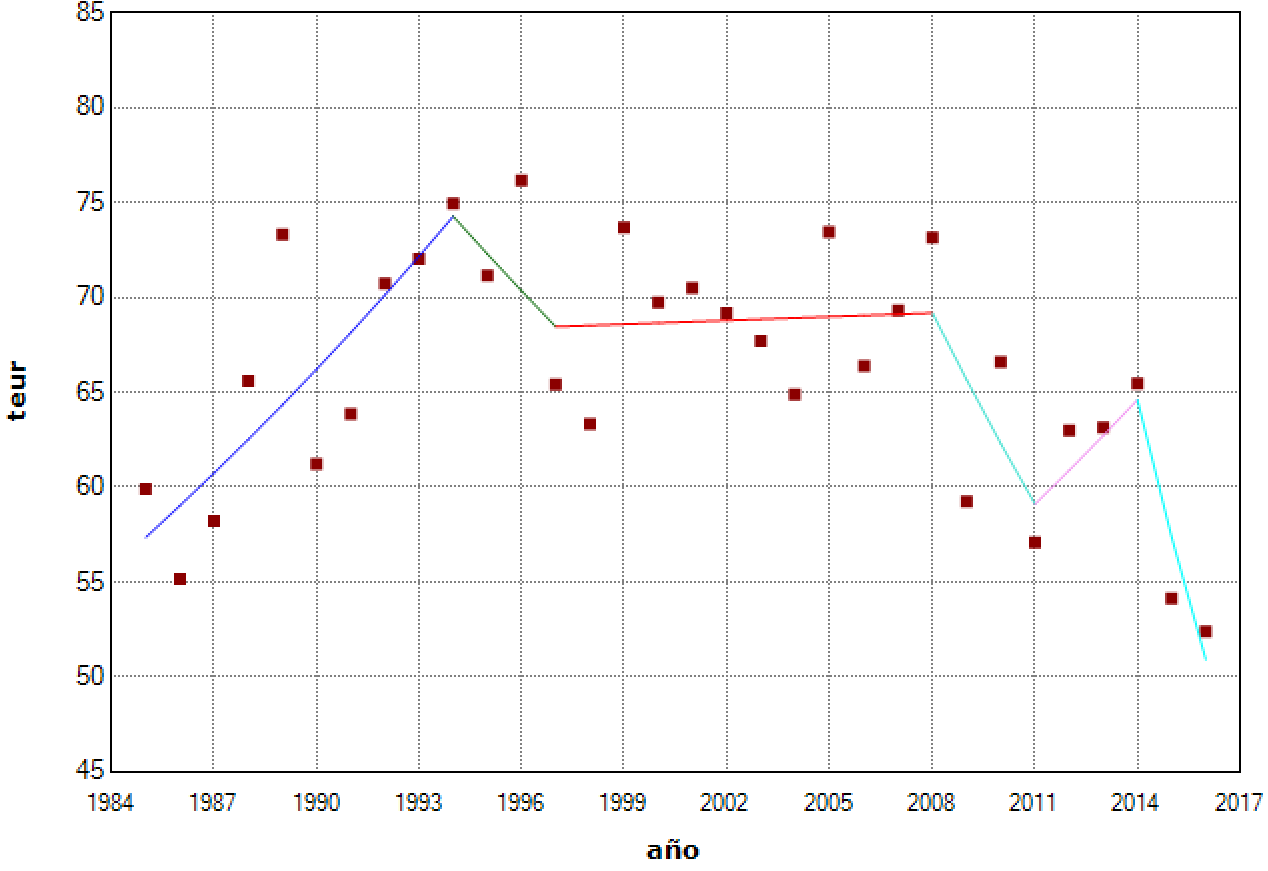
\includegraphics[width=\textwidth]{images/jpo5.png}
			\end{figure}
		\end{column}
	\end{columns}

	\pause
	\vspace{-110pt}
	\begin{columns}
		\begin{column}{.5\textwidth}
			\begin{figure}
				\centering
				
\includegraphics[width=.4\textwidth]{images/check.png}
			\end{figure}
		\end{column}
		\begin{column}{.5\textwidth}
		\end{column}
	\end{columns}

\end{frame}

%--------------------------------------------------

\begin{frame}\frametitle{Series temporales - Tendencias}
	\begin{columns}
		\begin{column}{0.5\textwidth}
			\centering \normalsize 0 puntos de inflexión
			\begin{figure}
				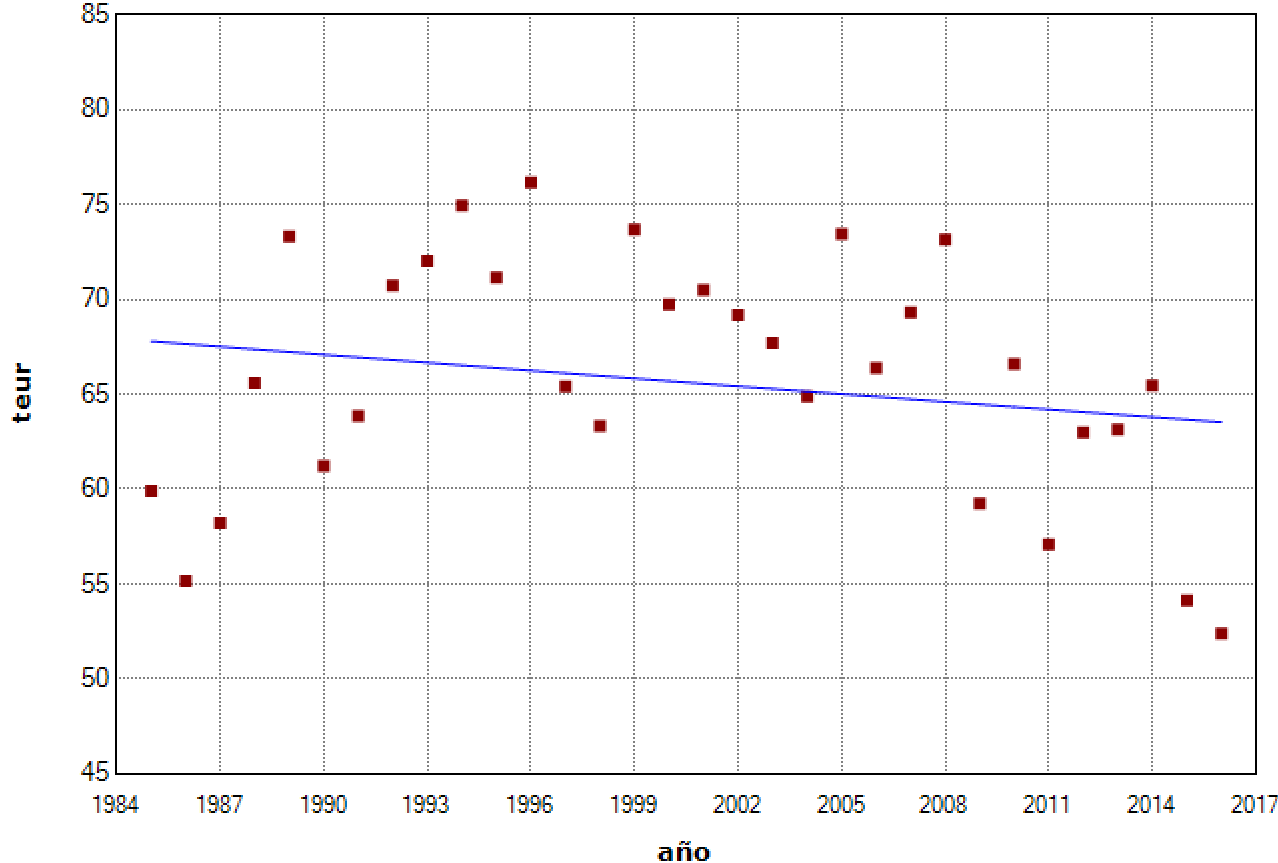
\includegraphics[width=\textwidth]{images/jpo0.png}
			\end{figure}
			
		\end{column}
		\large{\textbf{vs}}
		\begin{column}{0.5\textwidth}
			\centering \normalsize 4 puntos de inflexión
			\begin{figure}
				\centering
				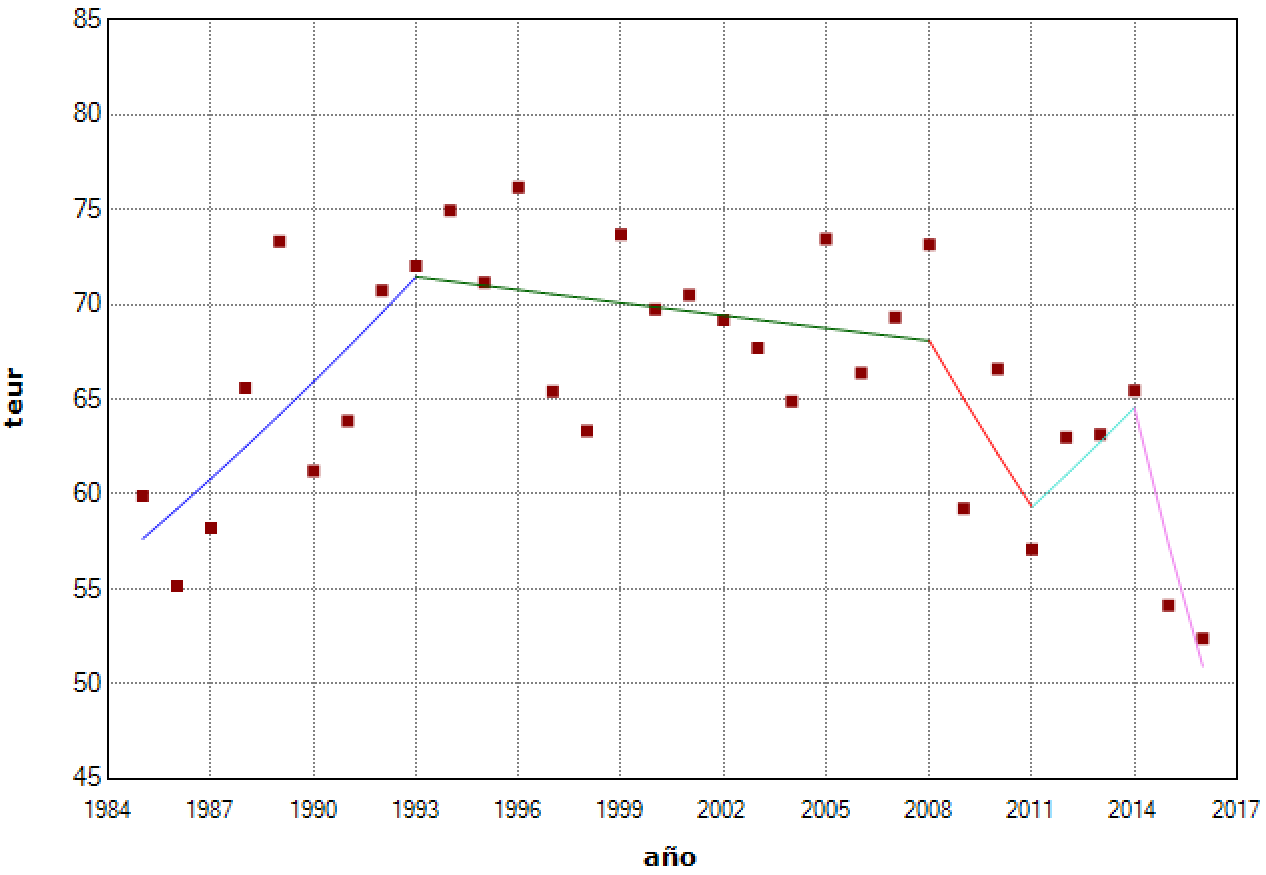
\includegraphics[width=\textwidth]{images/jpo4.png}
			\end{figure}
		\end{column}
	\end{columns}

	\pause
	\vspace{-110pt}
	\begin{columns}
		\begin{column}{.5\textwidth}
			\begin{figure}
				\centering
				
\includegraphics[width=.4\textwidth]{images/check.png}
			\end{figure}
		\end{column}
		\begin{column}{.5\textwidth}
		\end{column}
	\end{columns}
\end{frame}

%--------------------------------------------------

\begin{frame}\frametitle{Series temporales - Tendencias}
	\begin{columns}
		\begin{column}{0.5\textwidth}
			\centering \normalsize 0 puntos de inflexión
			\begin{figure}
				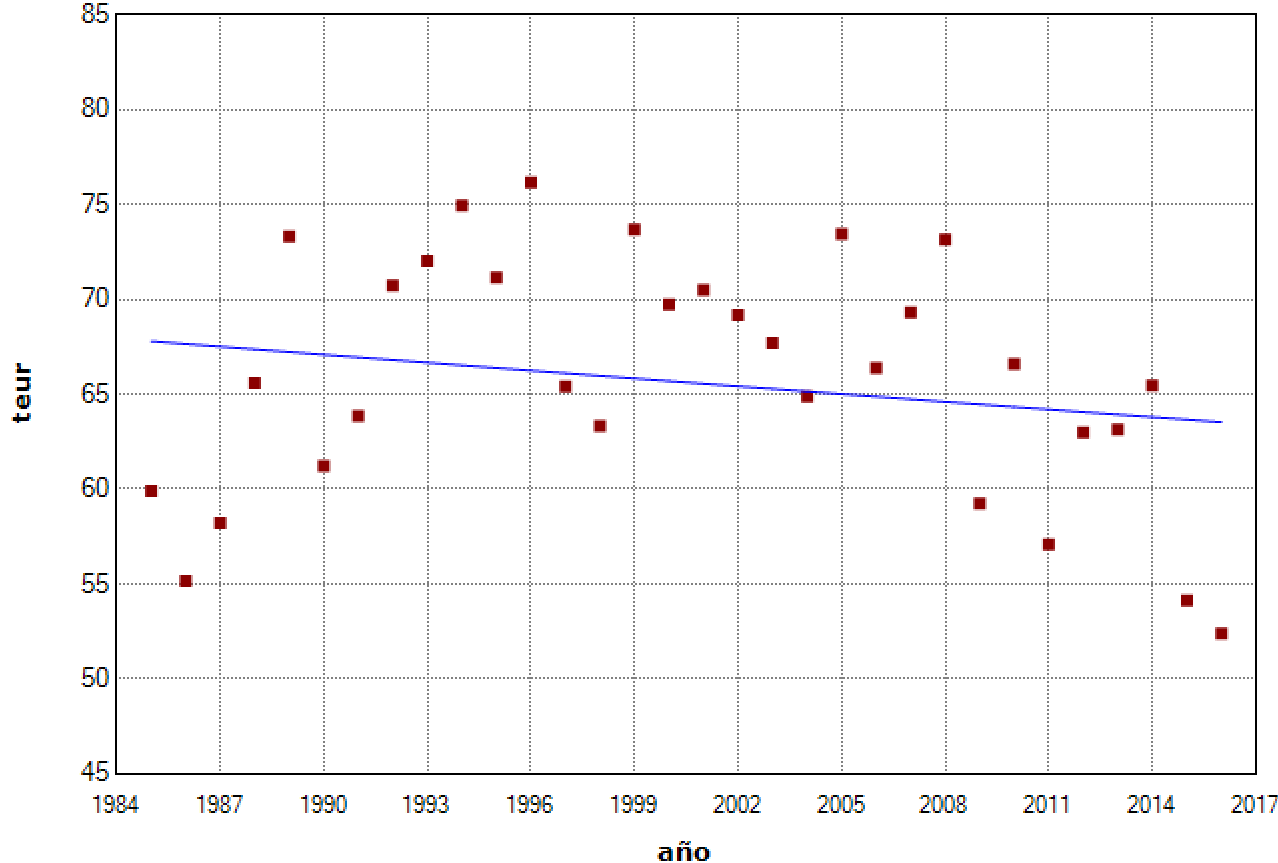
\includegraphics[width=\textwidth]{images/jpo0.png}
			\end{figure}
			
		\end{column}
		\large{\textbf{vs}}
		\begin{column}{0.5\textwidth}
			\centering \normalsize 3 puntos de inflexión
			\begin{figure}
				\centering
				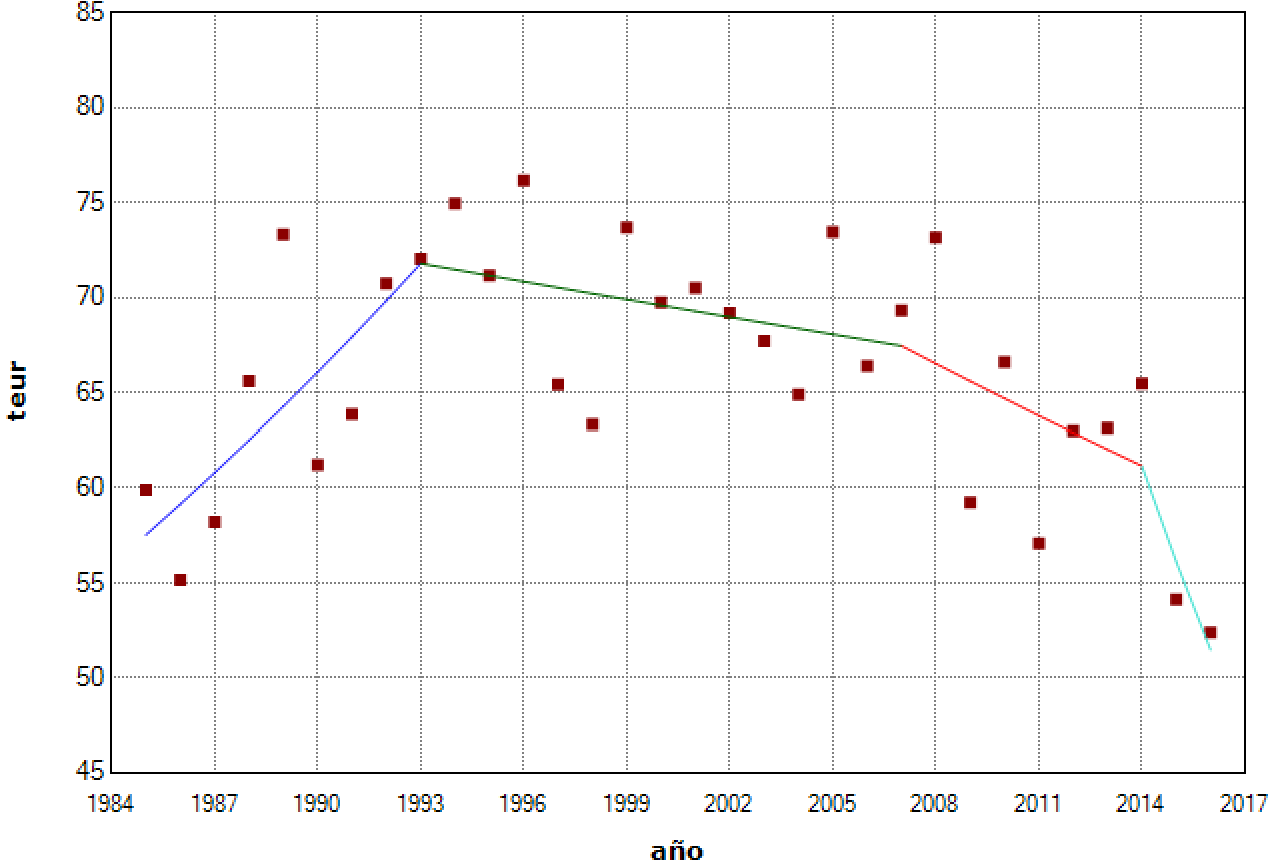
\includegraphics[width=\textwidth]{images/jpo3.png}
			\end{figure}
		\end{column}
	\end{columns}

	\pause
	\vspace{-110pt}
	\begin{columns}
		\begin{column}{.5\textwidth}
			\begin{figure}
				\centering
				
\includegraphics[width=.4\textwidth]{images/check.png}
			\end{figure}
		\end{column}
		\begin{column}{.5\textwidth}
		\end{column}
	\end{columns}

\end{frame}

%--------------------------------------------------

\begin{frame}\frametitle{Series temporales - Tendencias}
	\begin{columns}
		\begin{column}{0.5\textwidth}
			\centering \normalsize 0 puntos de inflexión
			\begin{figure}
				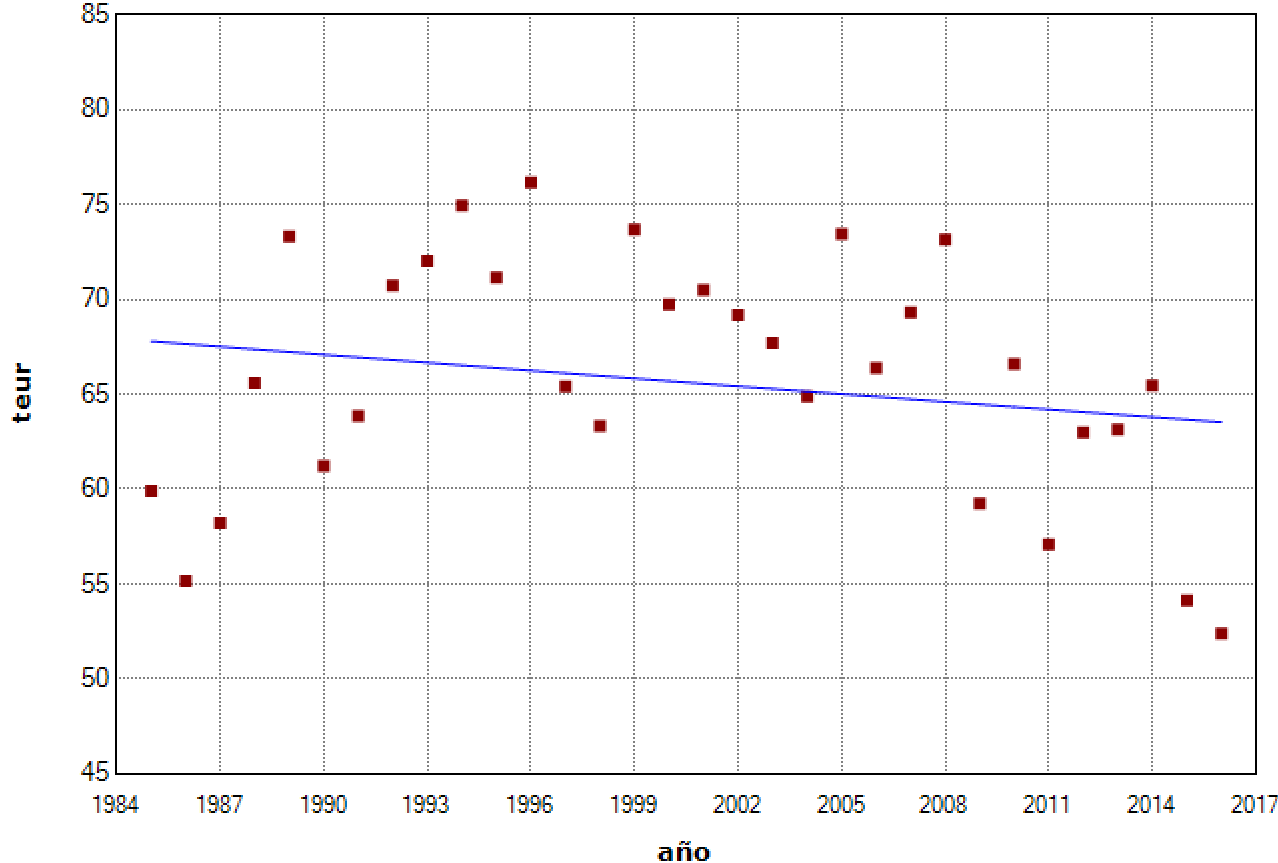
\includegraphics[width=\textwidth]{images/jpo0.png}
			\end{figure}
			
		\end{column}
		\large{\textbf{vs}}
		\begin{column}{0.5\textwidth}
			\centering \normalsize 2 puntos de inflexión
			\begin{figure}
				\centering
				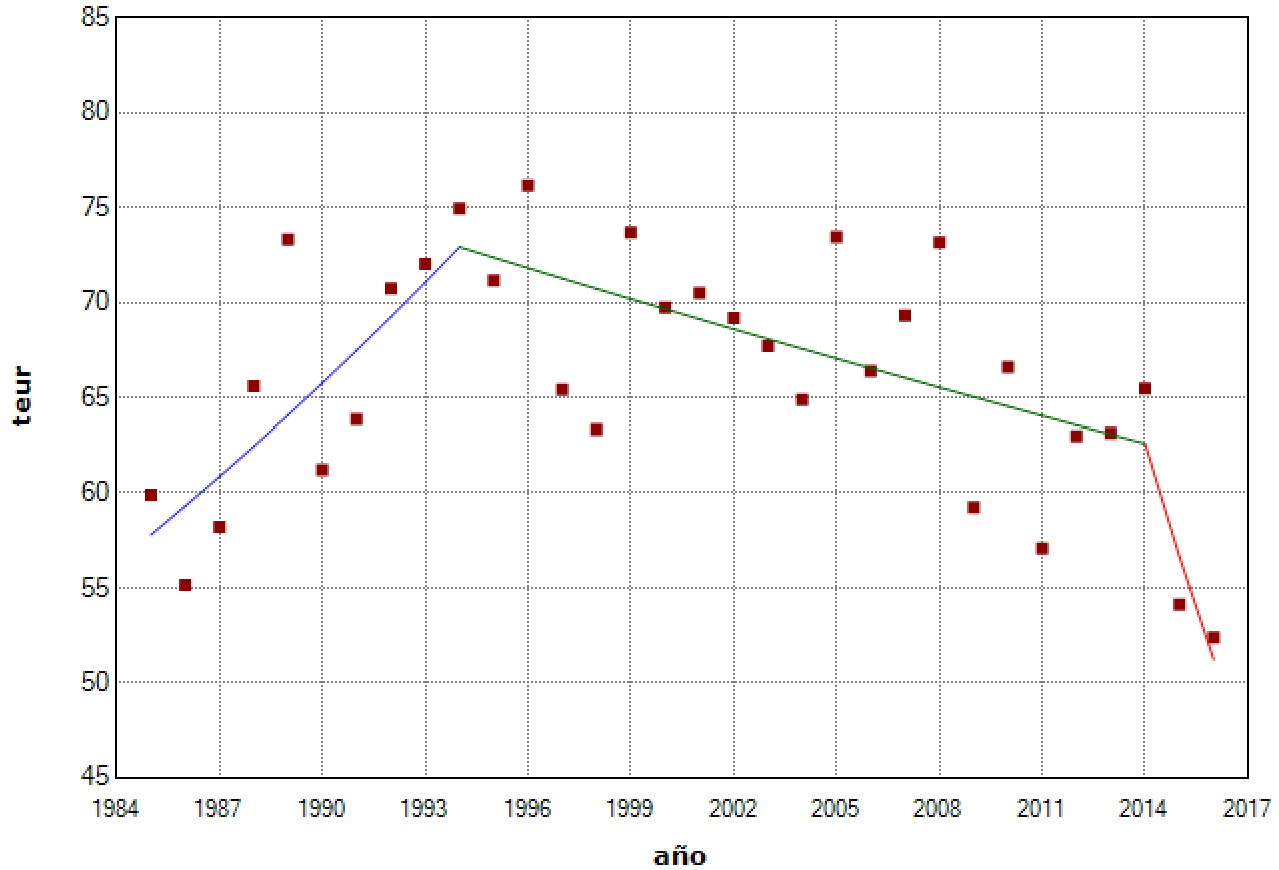
\includegraphics[width=\textwidth]{images/jpo2.png}
			\end{figure}
		\end{column}
	\end{columns}

	\pause
	\vspace{-110pt}
	\begin{columns}
		\begin{column}{.5\textwidth}
			\begin{figure}
				\centering
				
\includegraphics[width=.4\textwidth]{images/check.png}
			\end{figure}
		\end{column}
		\begin{column}{.5\textwidth}
		\end{column}
	\end{columns}

\end{frame}

%--------------------------------------------------

\begin{frame}\frametitle{Series temporales - Tendencias}
	\begin{columns}
		\begin{column}{0.5\textwidth}
			\centering \normalsize 0 puntos de inflexión
			\begin{figure}
				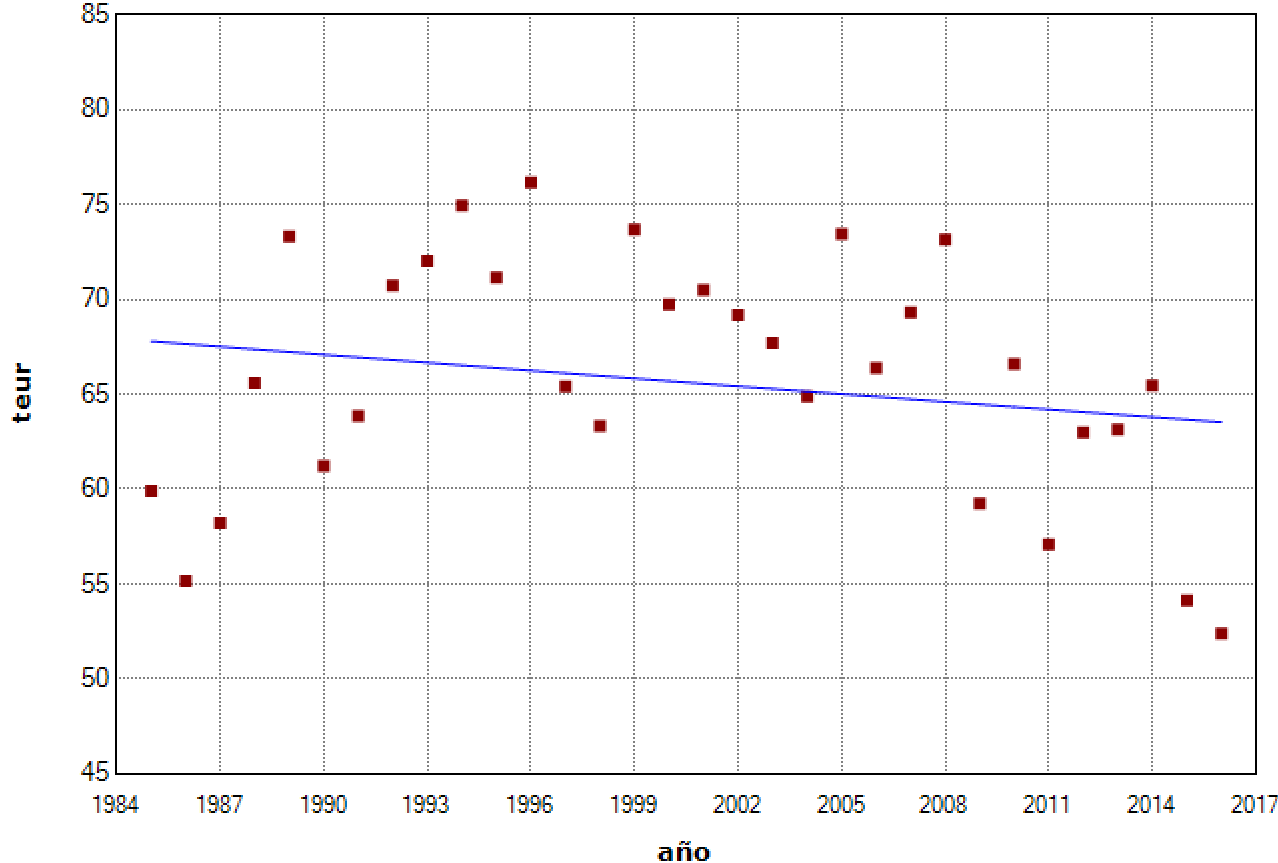
\includegraphics[width=\textwidth]{images/jpo0.png}
			\end{figure}
			
		\end{column}
		\large{\textbf{vs}}
		\begin{column}{0.5\textwidth}
			\centering \normalsize 1 punto de inflexión
			\begin{figure}
				\centering
				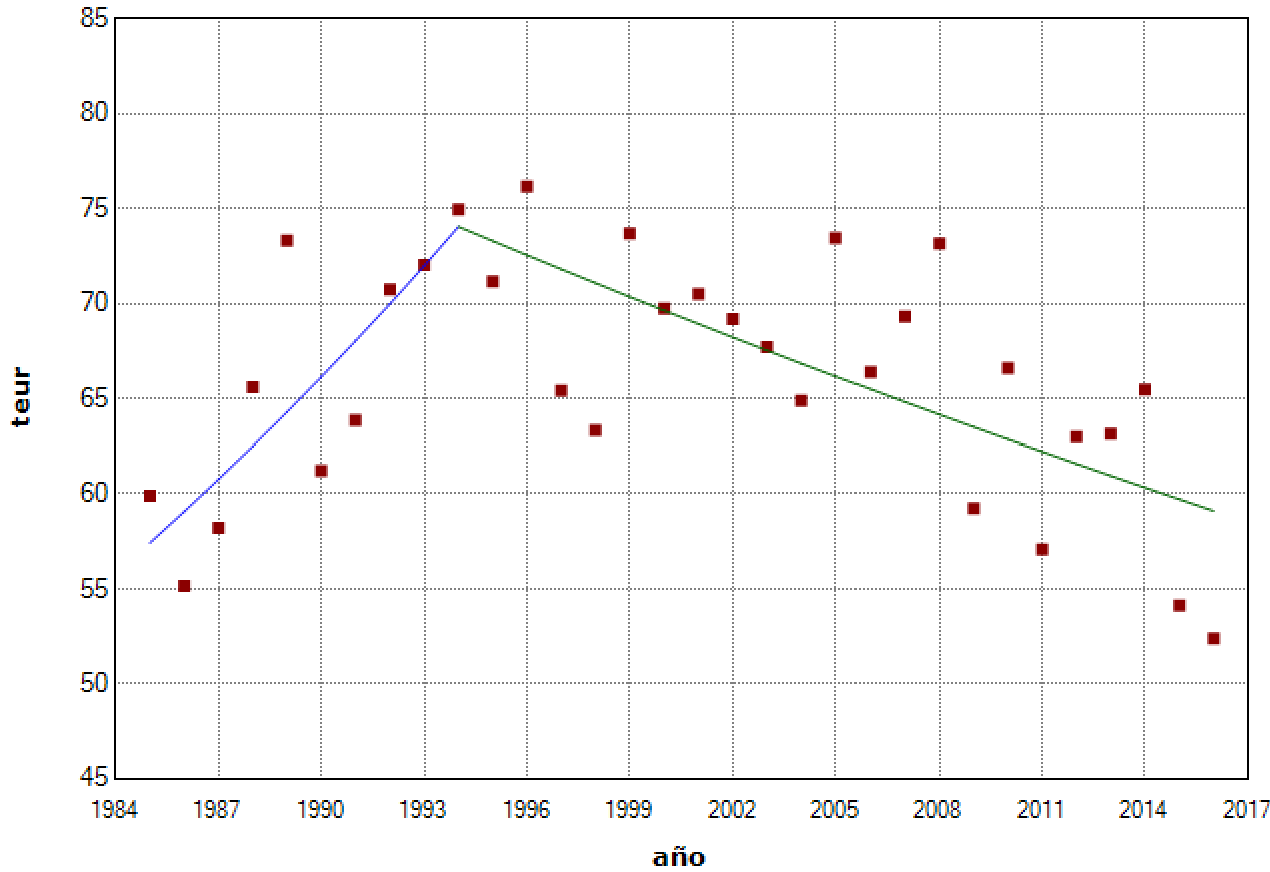
\includegraphics[width=\textwidth]{images/jpo1.png}
			\end{figure}
		\end{column}
	\end{columns}

	\pause
	\vspace{-110pt}
	\begin{columns}
		\begin{column}{.5\textwidth}
		\end{column}
		\begin{column}{.5\textwidth}
			\begin{figure}
				\centering
				\hspace{20pt}
\includegraphics[width=.4\textwidth]{images/check.png}
			\end{figure}
		\end{column}
	\end{columns}
\end{frame}

%--------------------------------------------------

\begin{frame}\frametitle{Series temporales - Tendencias}
	\centering
	Incidencia de cáncer de pulmón en hombres. Provincia de Granada, 1985-2016.
	\begin{figure}
		\centering
		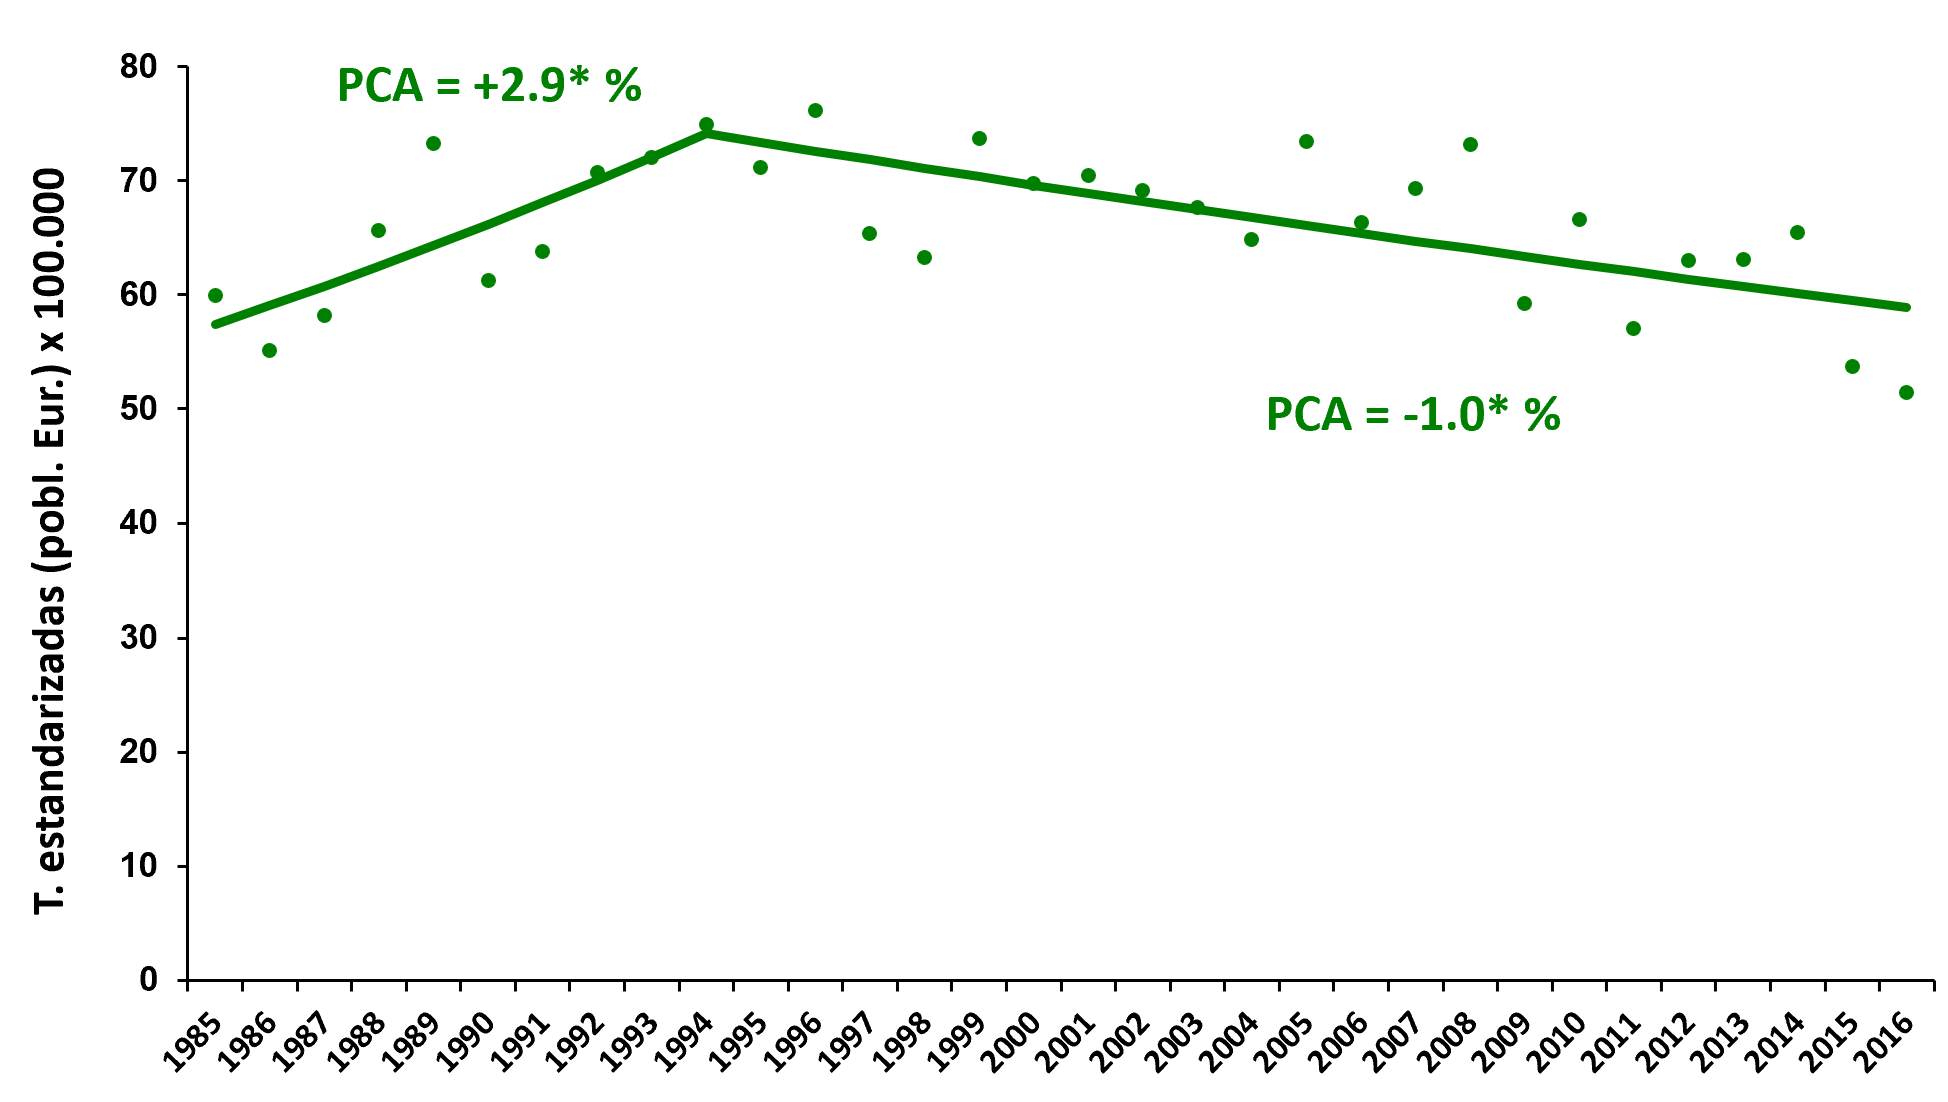
\includegraphics[width=\textwidth]{images/tendencias_pulmon1.png}
	\end{figure}
\end{frame}

%--------------------------------------------------

\begin{frame}\frametitle{Series temporales}
	\begin{block}{Series temporales}
		\begin{enumerate}
			\item Tendencias de la incidencia de cáncer\\[2ex]
			\item \textbf{Proyecciones de la incidencia de cáncer}\\[2ex]
			\item Estimaciones de la incidencia de cáncer\\[2ex]
		\end{enumerate}
	\end{block}
\end{frame}

%--------------------------------------------------

\begin{frame}\frametitle{Series temporales - Proyecciones}
	\footnotesize{Incidencia del total del cáncer excepto piel no melanoma. Provincia de Granada, 1985-2016.}
	\begin{figure}
		\centering
		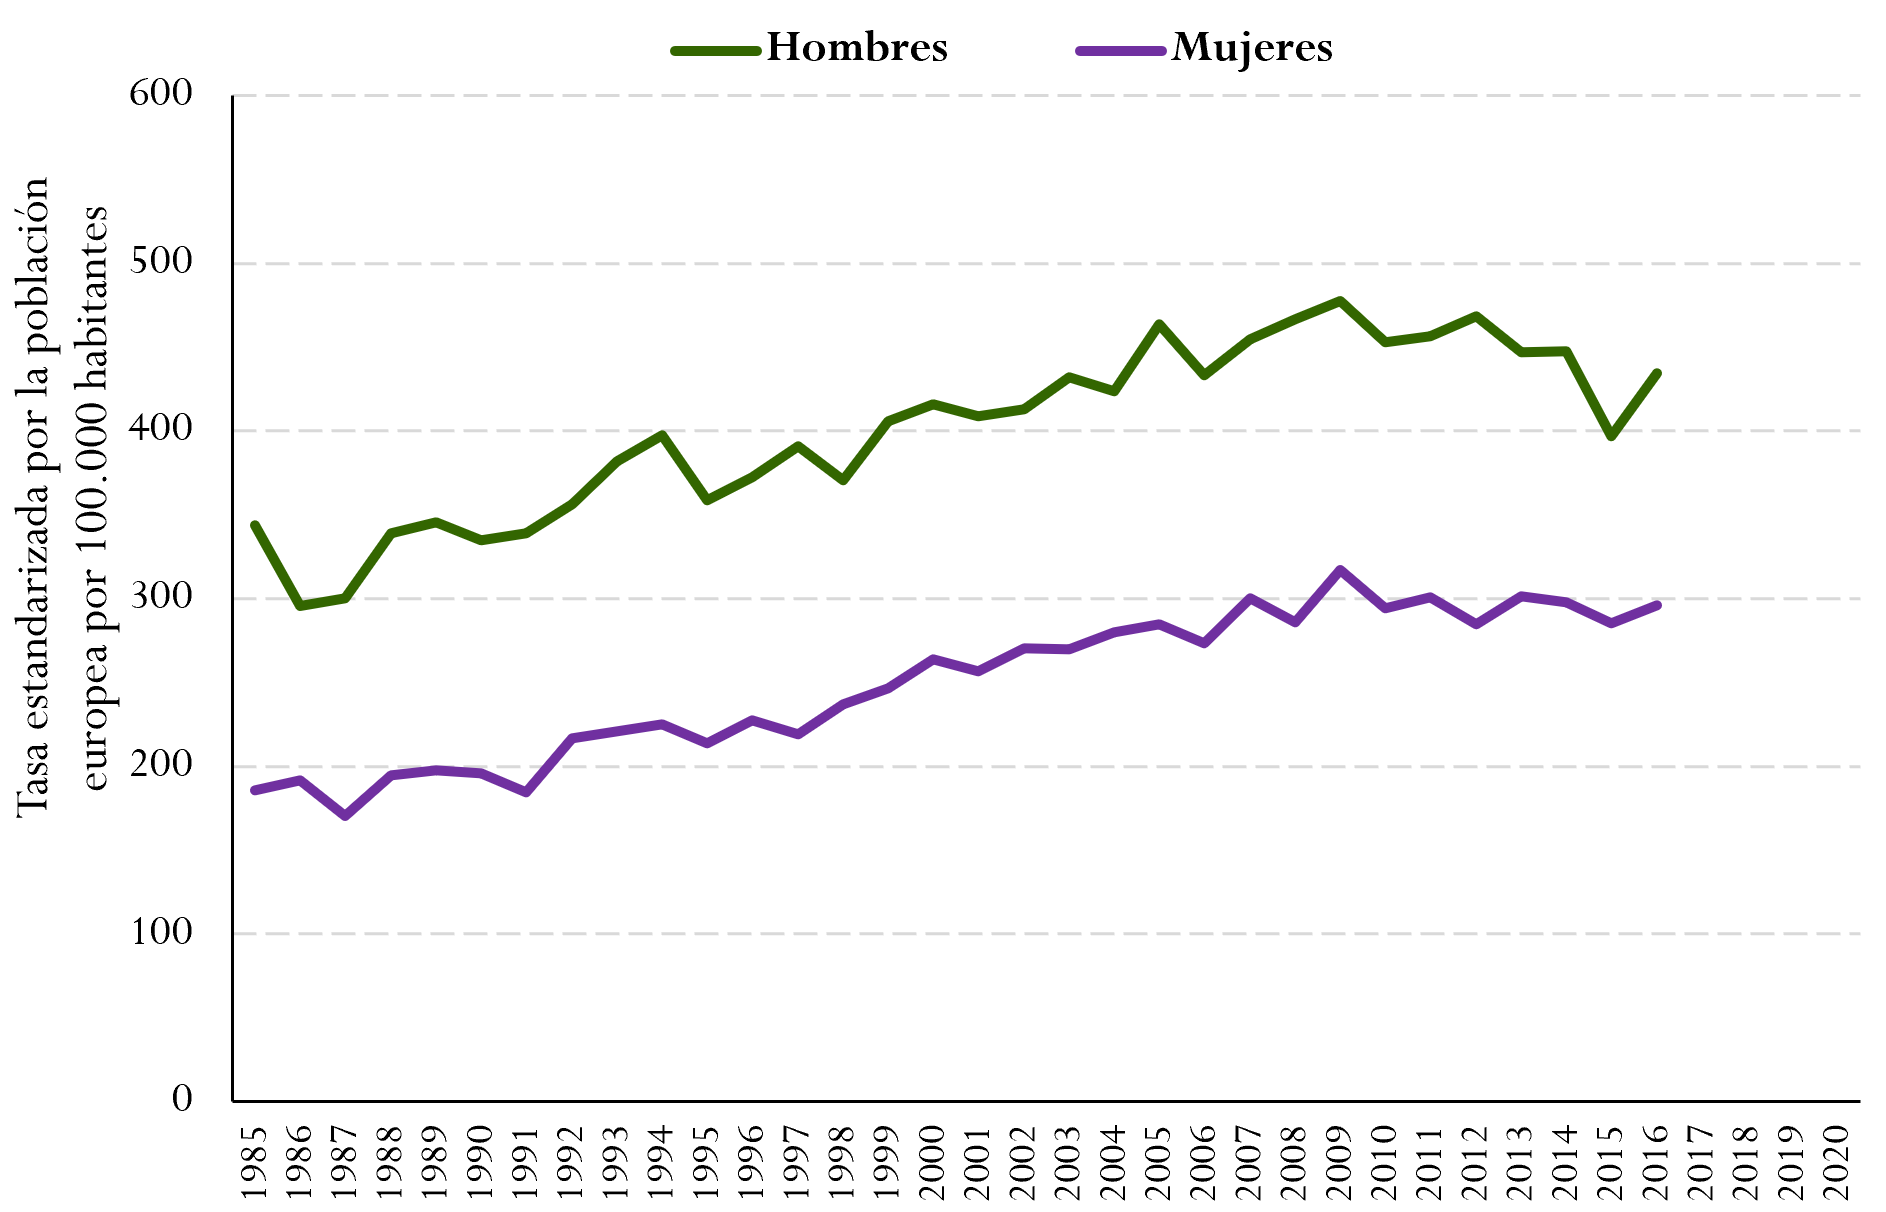
\includegraphics[width=0.9\textwidth]{images/proyecciones0.png}
	\end{figure}	
\end{frame}

%--------------------------------------------------

\begin{frame}\frametitle{Series temporales - Proyecciones}
	\vspace{-20pt}
	\centering
	$$log(\text{CASOS}) = \alpha + \beta_0 \text{AÑO} + \sum_{i = 1}^{18} \beta_i \text{EDAD}_i + log(\text{POBLACIÓN})$$
	\vspace{-10pt}
	\begin{figure}
		\centering
		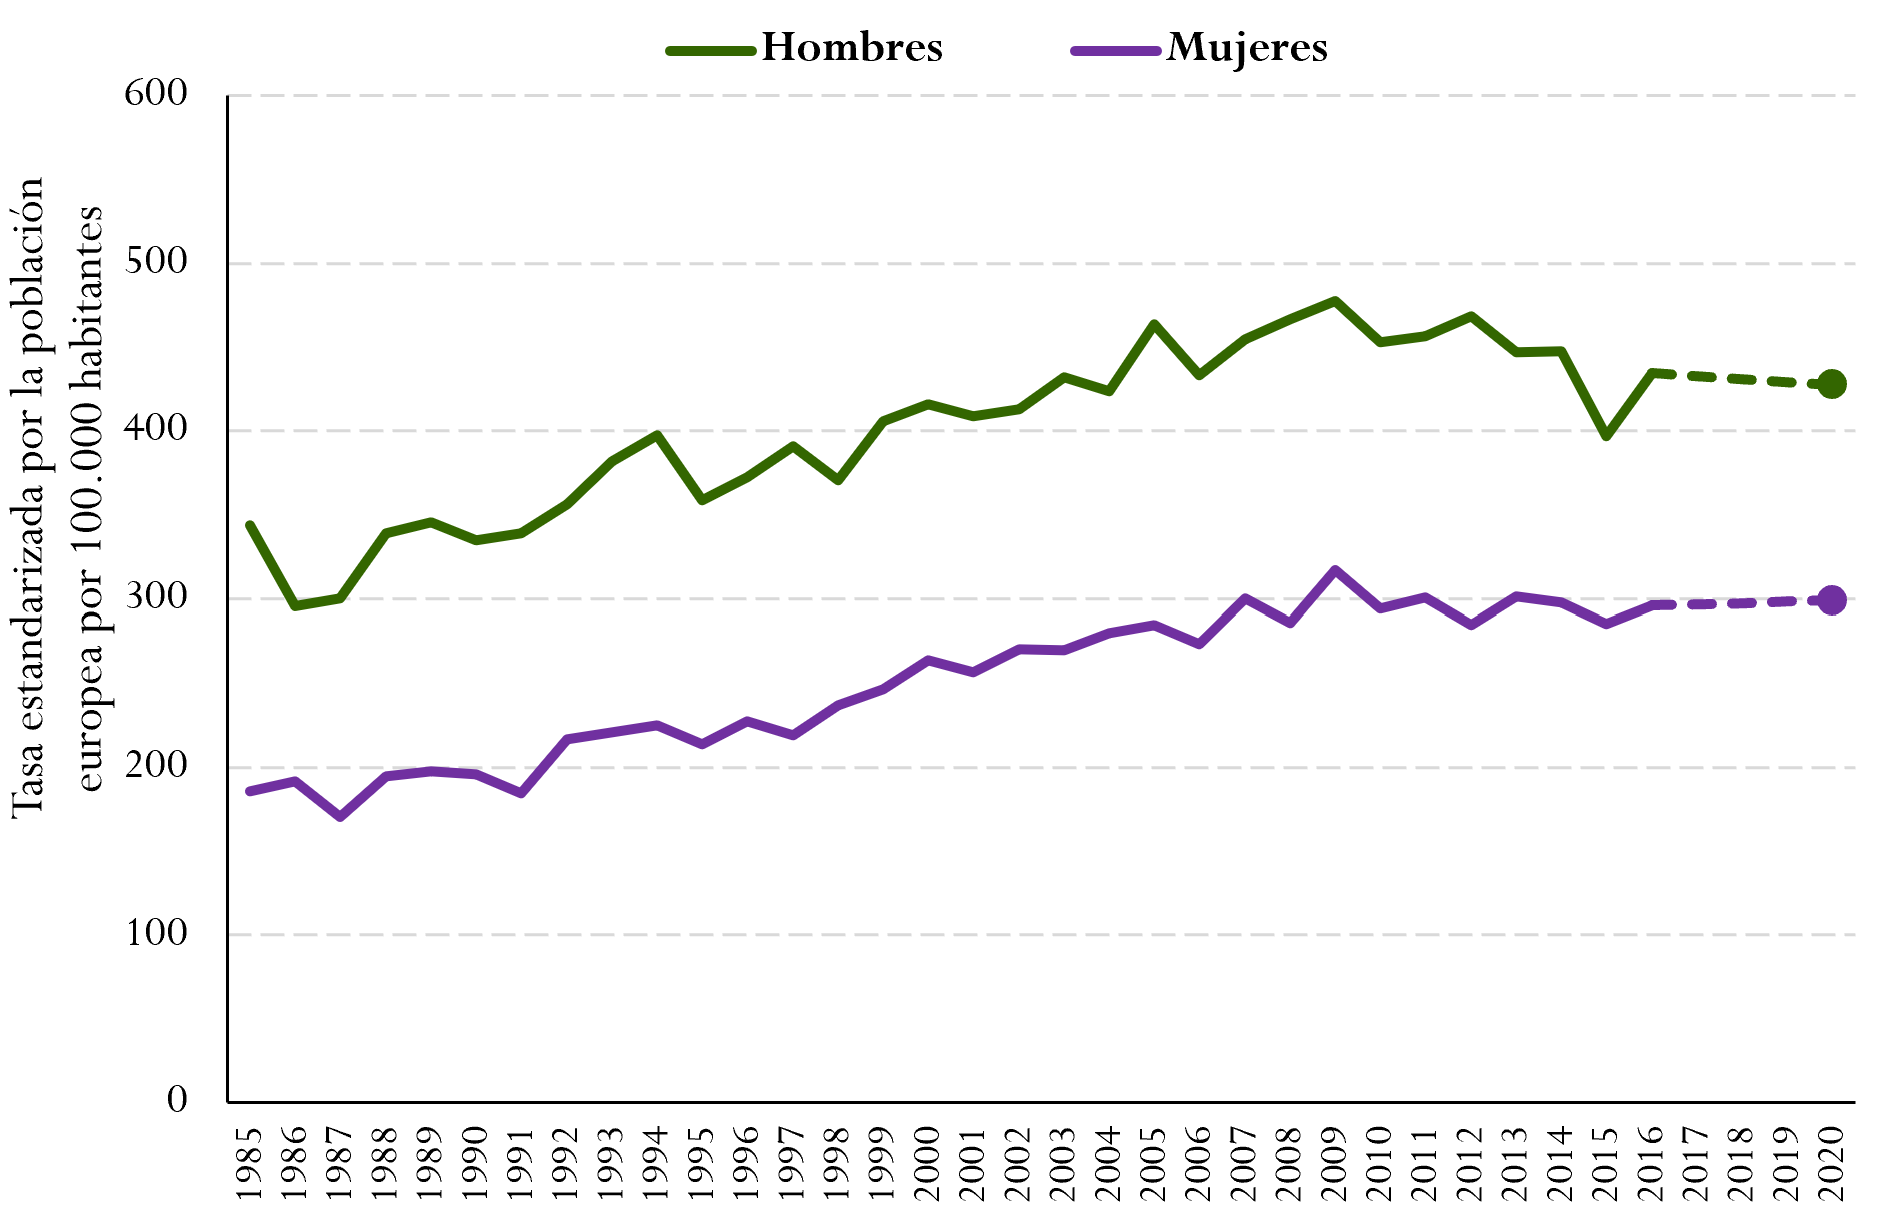
\includegraphics[width=0.9\textwidth]{images/proyecciones1.png}
	\end{figure}
\end{frame}

%--------------------------------------------------

\begin{frame}\frametitle{Series temporales}
	\begin{block}{Series temporales}
		\begin{enumerate}
			\item Tendencias de la incidencia de cáncer\\[2ex]
			\item Proyecciones de la incidencia de cáncer\\[2ex]
			\item \textbf{Estimaciones de la incidencia de cáncer}\\[2ex]
		\end{enumerate}
	\end{block}
\end{frame}

%--------------------------------------------------

\begin{frame}\frametitle{Series temporales - Estimaciones}
	\vspace{-20pt}
	\begin{columns}
		\begin{column}{0.5\textwidth}
			\begin{figure}
				\centering
				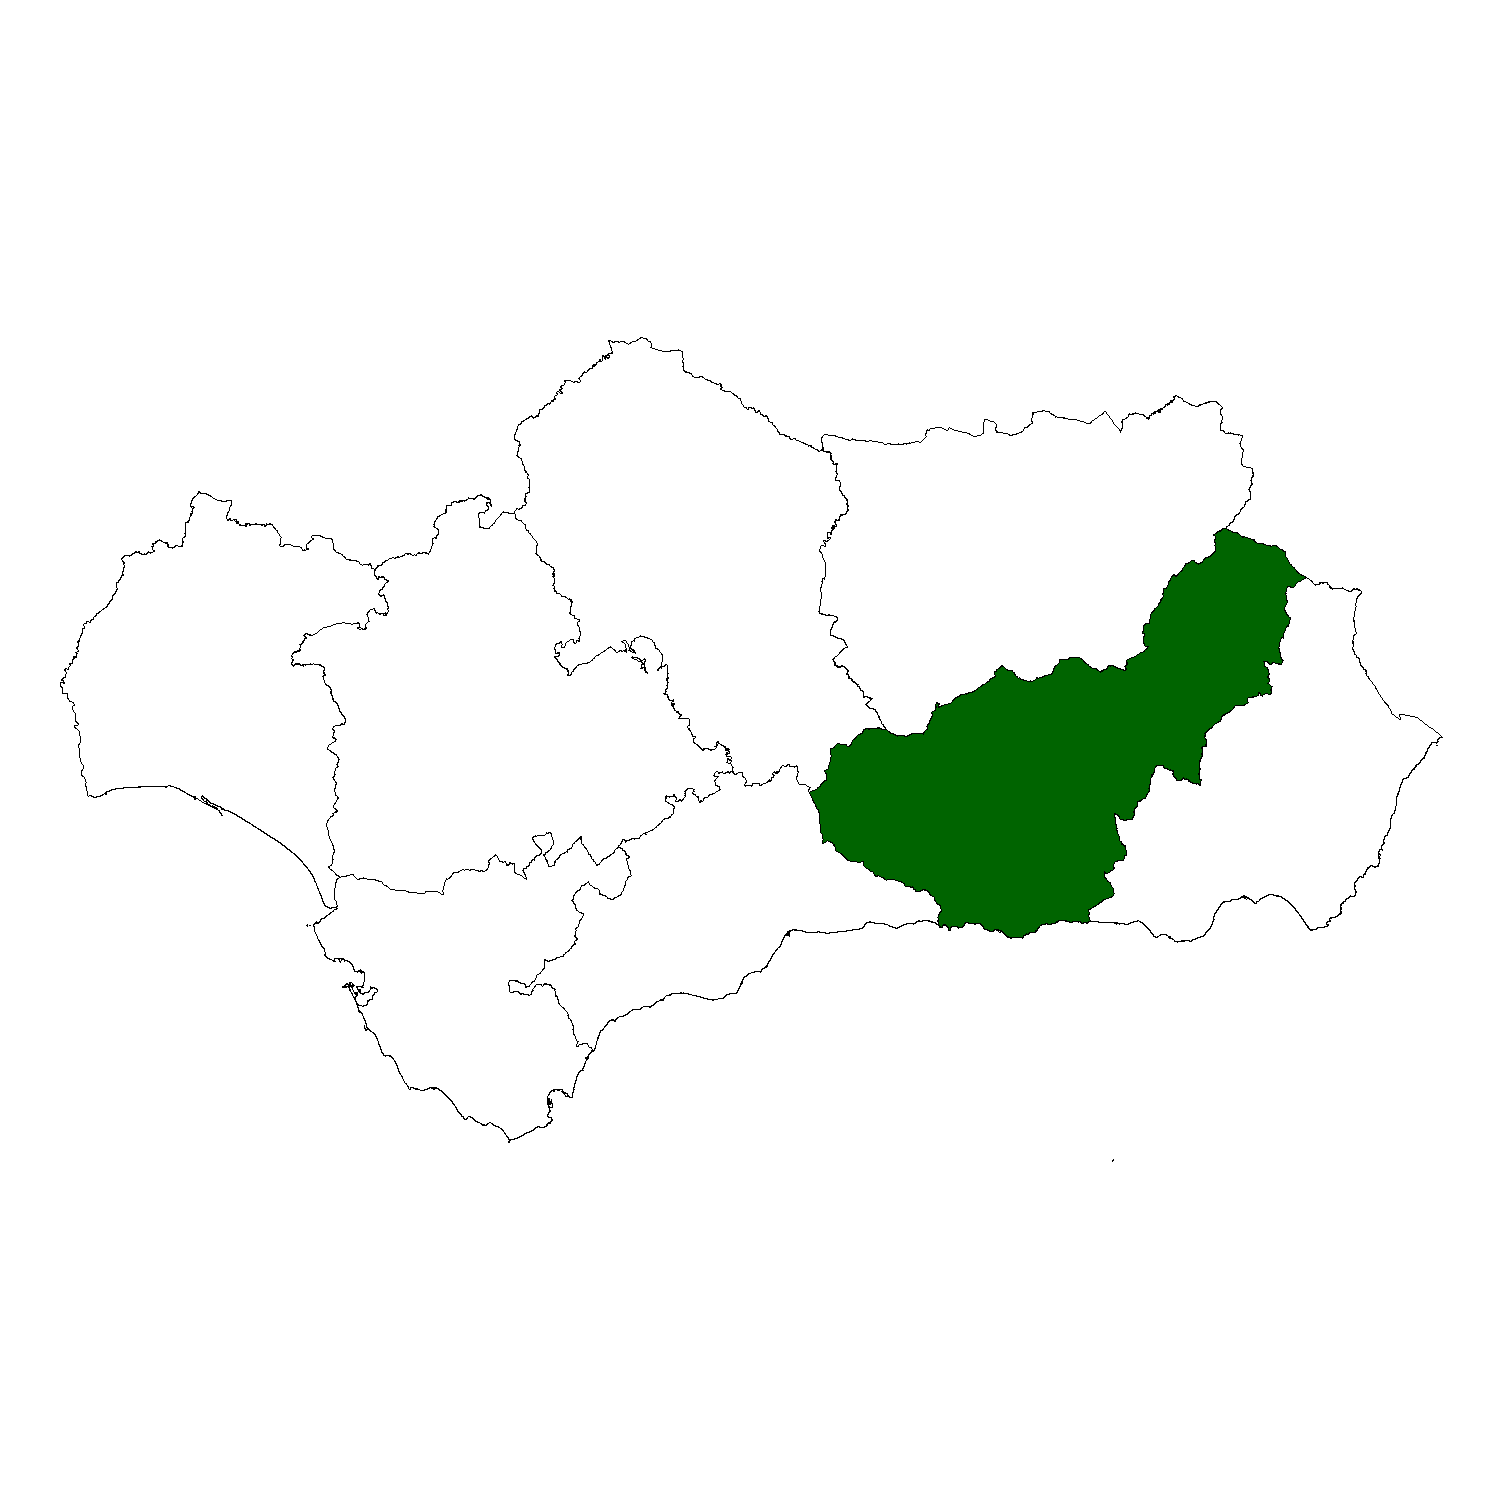
\includegraphics[width=0.9\textwidth]{images/granada.png}
			\end{figure}
		\end{column}
	\pause
		\Huge{\textbf{$\Rightarrow$}}
		\begin{column}{0.5\textwidth}
			\begin{figure}
				\centering
				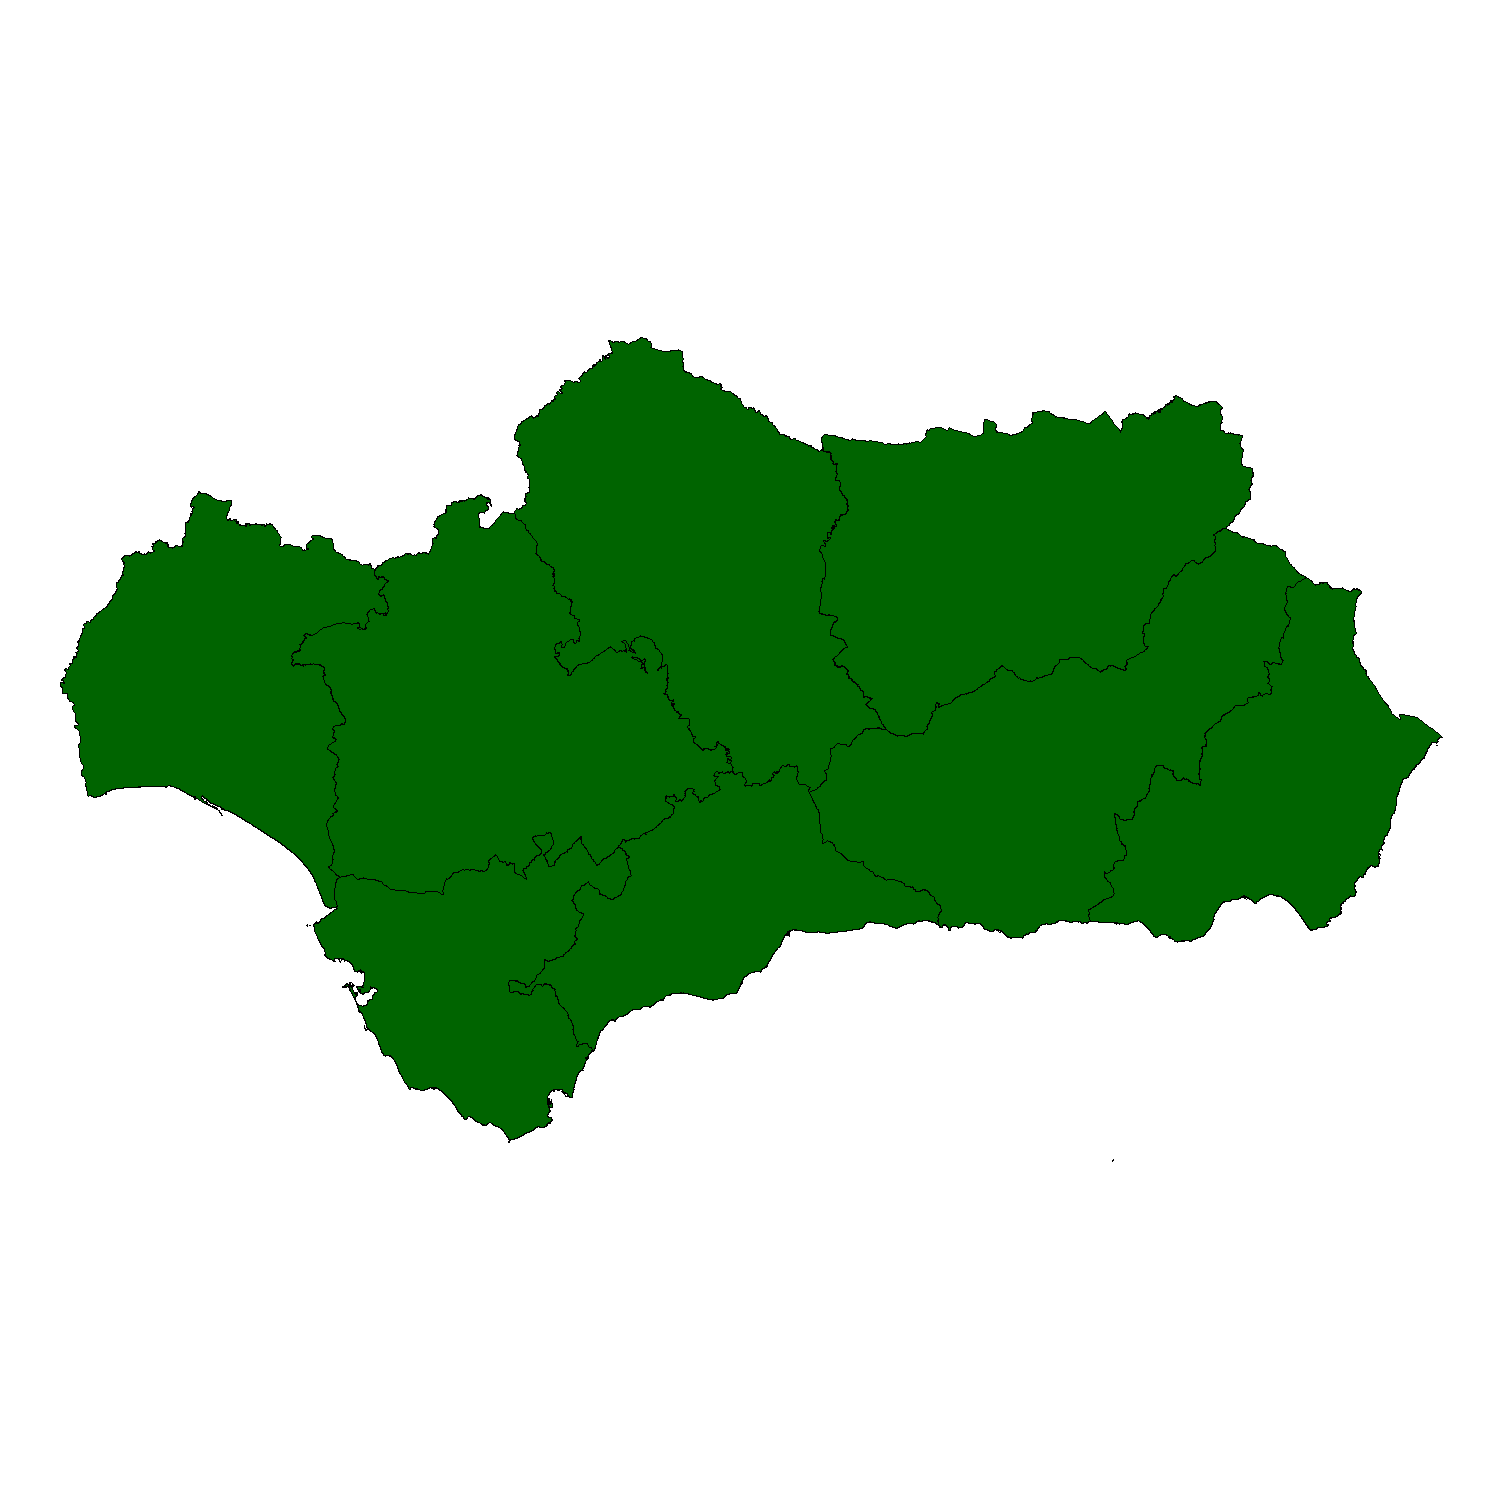
\includegraphics[width=0.9\textwidth]{images/andalucia.png}
			\end{figure}
		\end{column}
	\end{columns}

	\centering
	Se estima la incidencia en Andalucía usando \textbf{los datos de Granada} y varios métodos estadísticos (\textbf{cadenas de Markov-Montecarlo}, \textbf{modelos edad-periodo-cohorte}, \textbf{modelos lineales generalizados mixtos}, \textbf{suavizado exponencial} ...)
\end{frame}

%--------------------------------------------------

\begin{frame}\frametitle{Series temporales - Estimaciones}
	\begin{columns}
		\begin{column}{0.5\textwidth}
			\begin{figure}
				\centering
				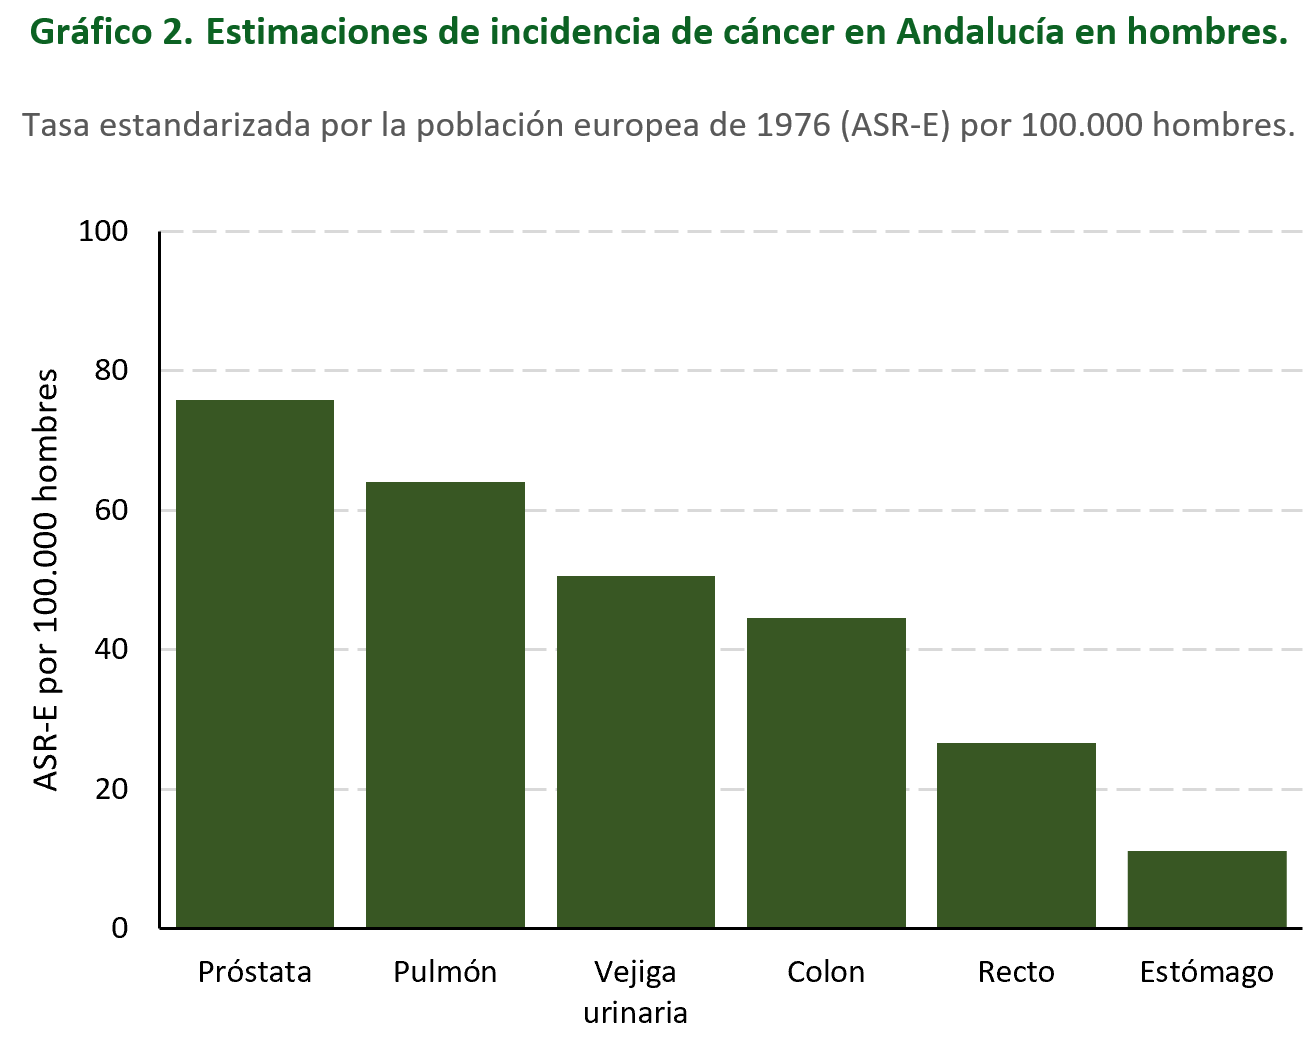
\includegraphics[width=\textwidth]{images/estimaciones_hombres.png}
			\end{figure}
		\end{column}
		\begin{column}{0.5\textwidth}
			\begin{figure}
				\centering
				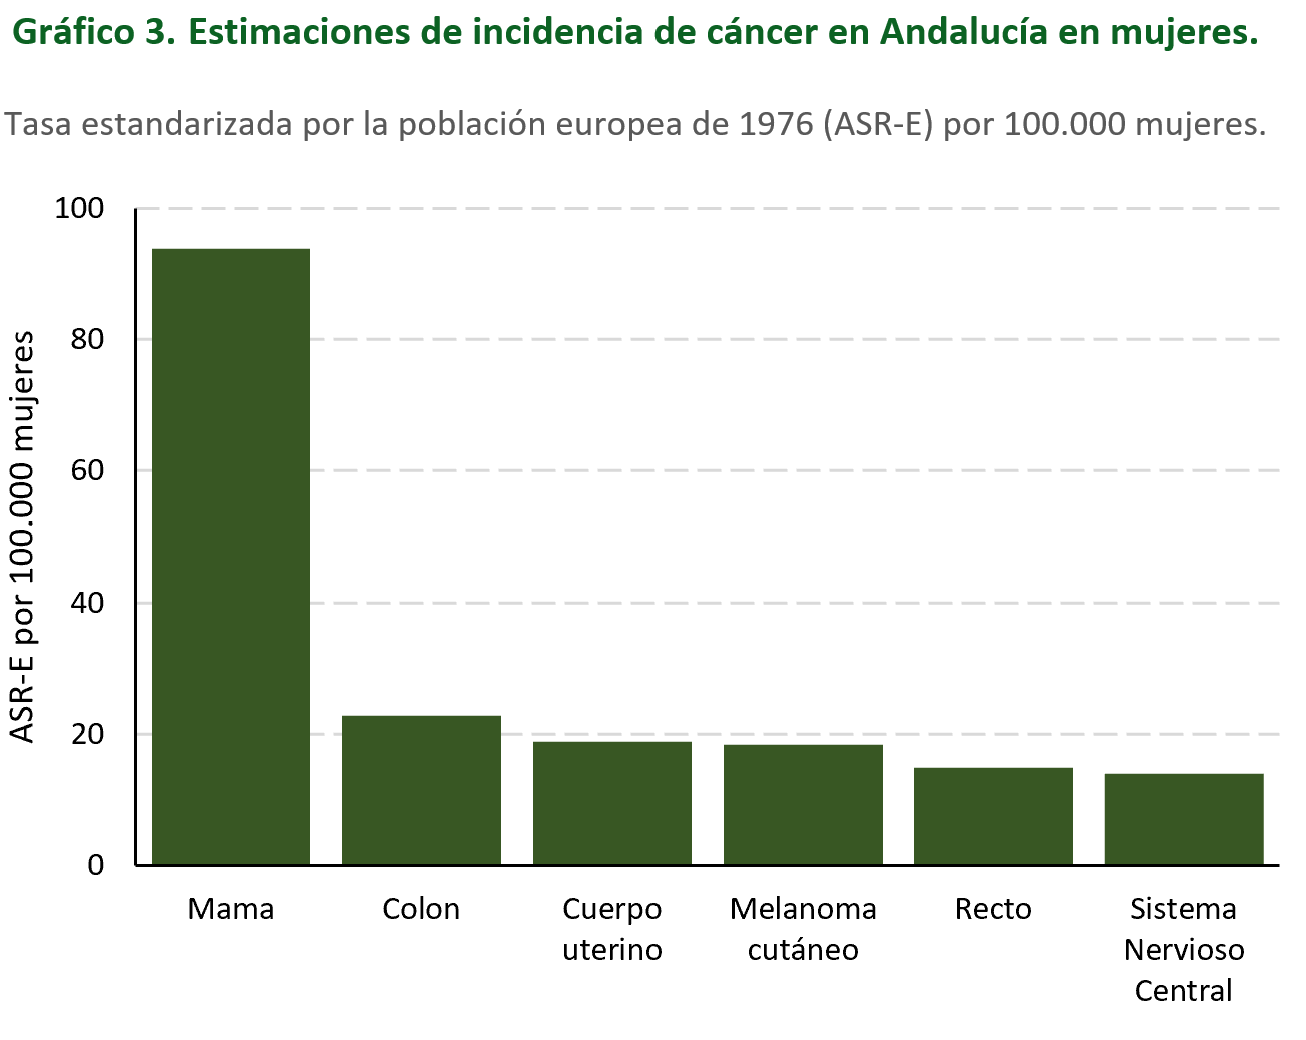
\includegraphics[width=\textwidth]{images/estimaciones_mujeres.png}
			\end{figure}
		\end{column}
	\end{columns}
\end{frame}

%--------------------------------------------------

\begin{frame}\frametitle{Series temporales - Estimaciones}
	\begin{columns}
		\begin{column}{0.5\textwidth}
			\begin{figure}
				\centering
				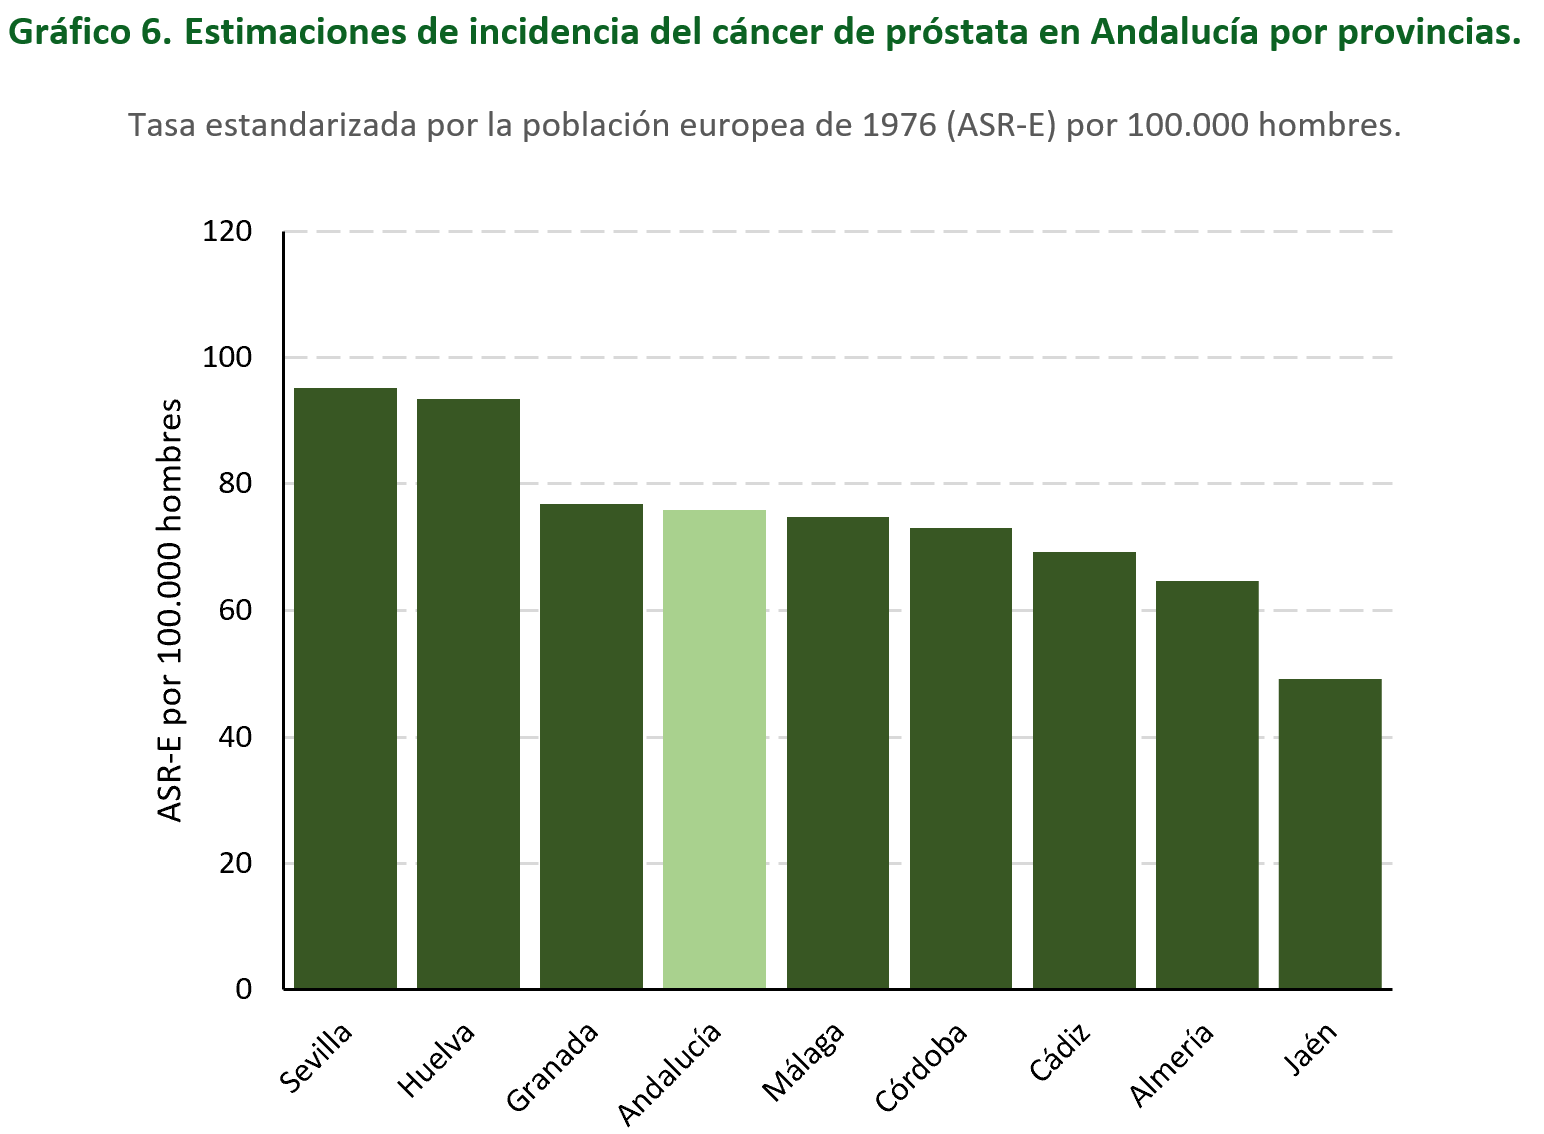
\includegraphics[width=.98\textwidth]{images/estimaciones_hombres2.png}
			\end{figure}
		\end{column}
		\begin{column}{0.5\textwidth}
			\begin{figure}
				\centering
				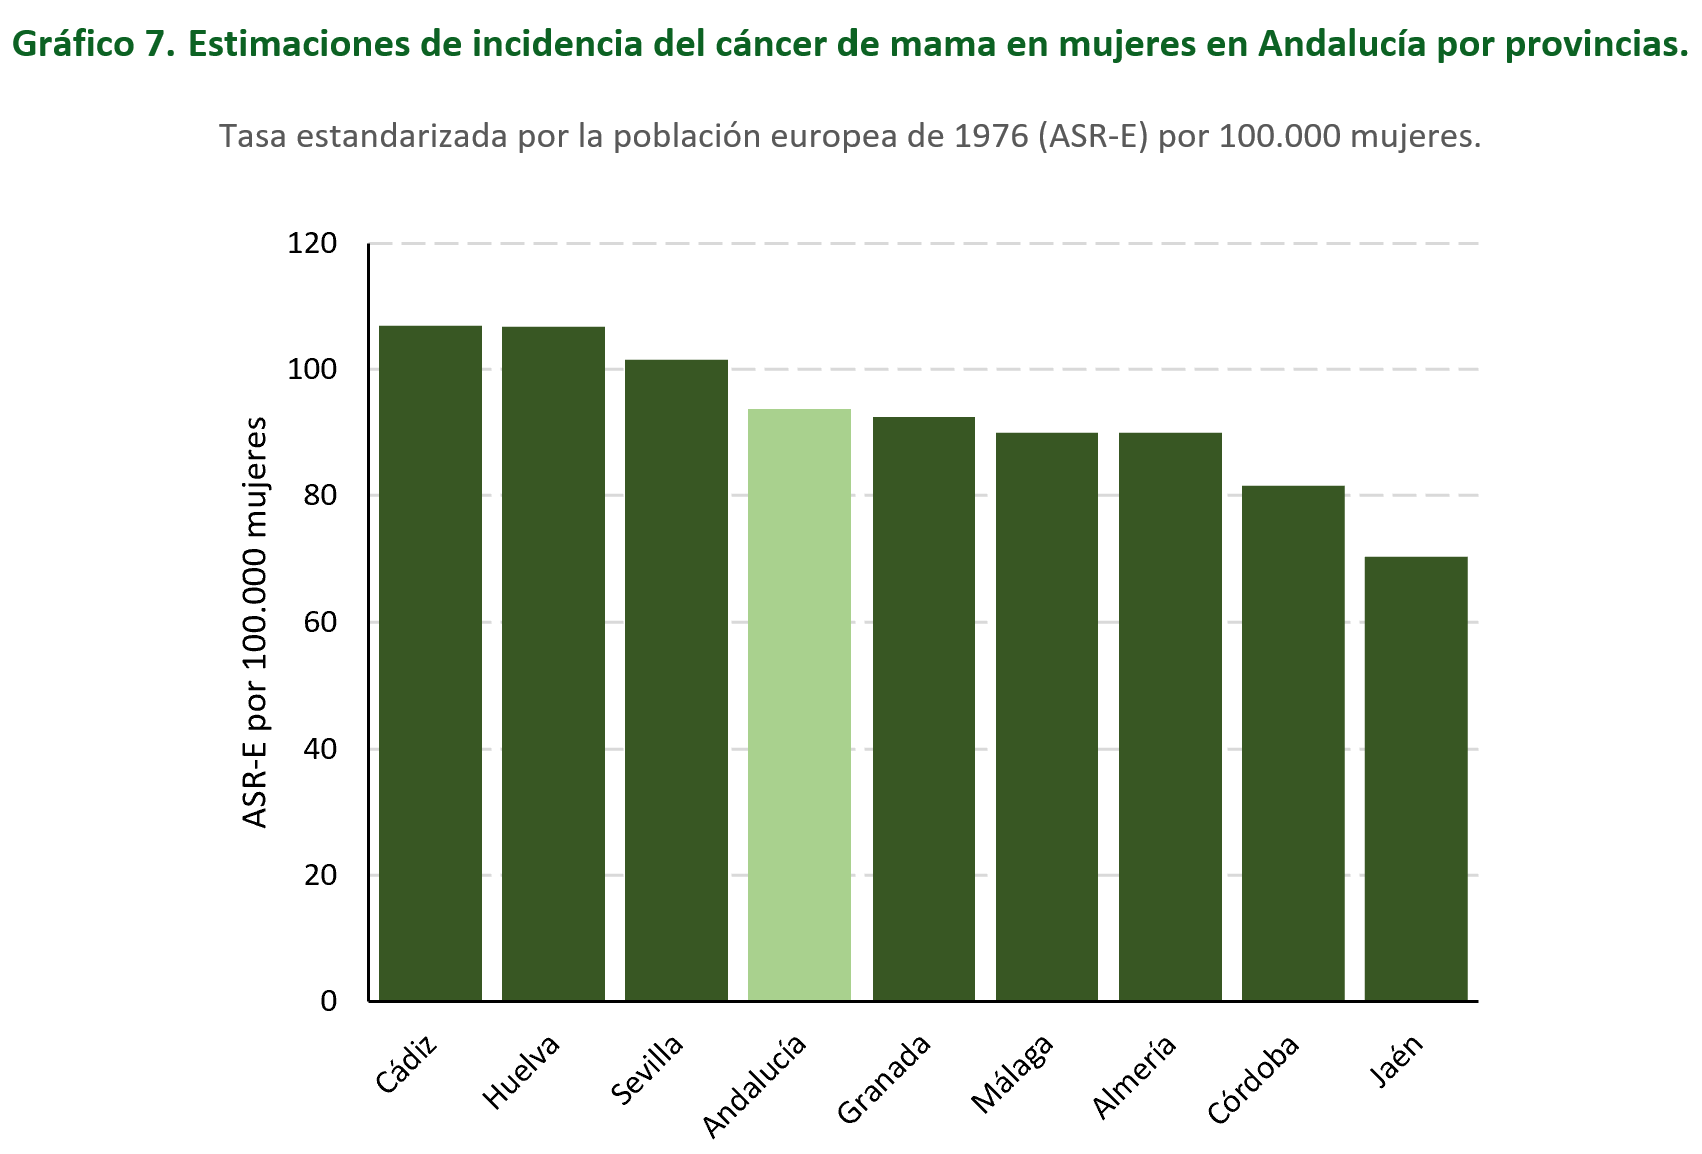
\includegraphics[width=1.02\textwidth]{images/estimaciones_mujeres2.png}
			\end{figure}
		\end{column}
	\end{columns}
\end{frame}

%--------------------------------------------------

\begin{frame}\frametitle{Series temporales - Estimaciones}
	\begin{columns}
		\begin{column}{0.4\textwidth}
			\begin{figure}
				\centering
				
\includegraphics[width=\textwidth]{images/tfm_matematicas.png}
			\end{figure}
		\end{column}
		\begin{column}{0.6\textwidth}
			\begin{figure}
				\centering
				\includegraphics[width=\textwidth]{images/tfm_matematicas2.png}
			\end{figure}
		\end{column}
	\end{columns}
\end{frame}

%--------------------------------------------------

\begin{frame}\frametitle{}
	\Large{\textbf{Índice}}\\[2ex]
	\normalsize
	\begin{enumerate}
		\item Epidemiología y cáncer\\[2ex]
		\item Herramientas\\[2ex]
		\item Series temporales \\[2ex]
		\item \textbf{Machine learning}  \\[2ex]
		\item Análisis espacial \\[2ex]
	\end{enumerate}
\end{frame}

%--------------------------------------------------

\begin{frame}\frametitle{Machine learning}
	\begin{block}{Machine learning}
		\begin{itemize}
			\item Campo híbrido: Estadística + Informática + Matemáticas... \\[2ex]
			\item Algoritmos de \textbf{selección de características}: elección de variables relevantes.\\[2ex]
			\item Algoritmos de \textbf{regresión} y \textbf{clasificación}.\\[2ex]
			\item Un ejemplo con R+\{KnowSeq\}...
		\end{itemize}
		\begin{figure}
			\centering
			\includegraphics[width=.15\textwidth]{images/06_logo_knowseq.png}			
		\end{figure}
		\vspace{-10pt}
		\centering
		\url{https://github.com/CasedUgr/KnowSeq}
	\end{block}
\end{frame}

%--------------------------------------------------

\begin{frame}\frametitle{Machine learning}
	\begin{itemize}
		\item 462 muestras de tejido de hígado.
		\item 404 identificados como tumores, 58 como tejido sano.
		\item +24.500 genes en cada muestra.
	\end{itemize}
	\textbf{Objetivo}: buscar genes que permitan ``clasificar" una muestra nueva como tumor o tejido sano.
	\begin{figure}
		\centering
		\includegraphics[width=.65\textwidth]{images/liver.jpg}
	\end{figure}
\end{frame}

%--------------------------------------------------

\begin{frame}\frametitle{Machine learning}
	\begin{figure}
		\centering
		\includegraphics[width=.75\textwidth]{images/07_higado_biclase_sankey.png}
	\end{figure}
\end{frame}

%--------------------------------------------------

\begin{frame}\frametitle{Machine learning}
	Con el conjunto de entrenamiento:
	\begin{figure}
		\centering
		\includegraphics[width=.6\textwidth]{images/15_higado_biclase_42_knn_heatmap_mejor_metodo.png}
	\end{figure}
\end{frame}

%--------------------------------------------------

\begin{frame}\frametitle{Machine learning}
	\begin{figure}
		\centering
		\includegraphics[width=.9\textwidth]{images/16_higado_biclase_43_knn_boxplots_mejor_metodo.png}
	\end{figure}
\end{frame}

%--------------------------------------------------

\begin{frame}\frametitle{Machine learning}
	Se entrena un modelo con 2 genes y se aplica al conjunto de test:
	\begin{figure}
		\centering
		\includegraphics[width=.9\textwidth]{images/17_higado_biclase_18_svm_matriz_confusion_mejor_metodo.png}
	\end{figure}
\end{frame}

%--------------------------------------------------
\begin{frame}\frametitle{}
	\Large{\textbf{Índice}}\\[2ex]
	\normalsize
	\begin{enumerate}
		\item Epidemiología y cáncer\\[2ex]
		\item Herramientas\\[2ex]
		\item Series temporales \\[2ex]
		\item Machine learning \\[2ex]
		\item \textbf{Análisis espacial} \\[2ex]
	\end{enumerate}
\end{frame}

%--------------------------------------------------

\begin{frame}\frametitle{Análisis espacial}
	\centering Estudio de John Snow sobre cólera.
	\begin{figure}
		\centering
		\includegraphics[width=.75\textwidth]{images/mapa_3.png}
	\end{figure}
\end{frame}

%--------------------------------------------------

\begin{frame}\frametitle{Análisis espacial}
	\begin{figure}
		\centering
		\includegraphics[width=.8\textwidth]{images/mapa_0.png}
	\end{figure}
	\begin{columns}
		\begin{column}{0.5\textwidth}
			\begin{figure}
				\centering
				\includegraphics[width=.9\textwidth]{images/mapa_1.png}
			\end{figure}
		\end{column}
		\begin{column}{0.5\textwidth}
			\begin{figure}
				\centering
				\includegraphics[width=.6\textwidth]{images/mapa_2.png}
			\end{figure}
		\end{column}
	\end{columns}
\end{frame}

%--------------------------------------------------

\begin{frame}\frametitle{Análisis espacial}
	\centering Índice de privación en Granada capital.
	\begin{figure}
		\centering
		\includegraphics[width=.9\textwidth]{images/maps_DI_zoom.png}
	\end{figure}
\end{frame}

%--------------------------------------------------

\begin{frame}\frametitle{Análisis espacial}
	\centering Incidencia de cáncer de pulmón en Granada capital.
	\begin{figure}
		\centering
		\includegraphics[width=.9\textwidth]{images/03_lung_ebs_zoom.png}
	\end{figure}
\end{frame}

%--------------------------------------------------

\begin{frame}\frametitle{}
	\begin{block}{Y mucho más...}
		\begin{itemize}
			\item Análisis espacial con distancia a \textbf{focos contaminantes}.
			\item \textbf{Epidemiología ambiental}. Factores de riesgo físicos (calor, ruido, radiaciones...), químicos (plaguicidas, metales...) y biológicos (virus, bacterias...).
			\item Estadísticas de cáncer \textbf{por municipios}.
			\item \textbf{Retrasos} diagnósticos.
			\item \textbf{Salud mental} en cáncer.
			\item Efectividad de programas de \textbf{screening}.
			\item \textbf{Costes} socio-económicos del cáncer.
			\item \textbf{Nutrición} y cáncer.
		\end{itemize}
	\end{block}
\end{frame}

%--------------------------------------------------

\begin{frame}\frametitle{}
	\begin{block}{Mensajes clave}
		\begin{itemize}
			\item \textbf{Programar} es muy importante y ayuda a \textbf{resolver problemas} y \textbf{automatizar procesos}.\\[2ex]
			\item Es difícil encontrar \textbf{personal de estadística especializado en investigación biomédica}. Se valora especialmente el grado de doctor.\\[2ex]
			\item \textbf{La investigación biosanitaria necesita estadísticos y estadísticas}.\\[2ex]
		\end{itemize}
	\end{block}
\end{frame}

%--------------------------------------------------

\begin{frame}[fragile]
	% Logos
	\begin{columns}
		\begin{column}{0.33\textwidth}
			\begin{figure}
				\centering
				\includegraphics[width=.9\textwidth]{logos/logo_ibs.jpg}
			\end{figure}
		\end{column}
		\begin{column}{0.33\textwidth}
			\begin{figure}
				\centering
				\includegraphics[width=.8\textwidth]{logos/logo_ugr.png}
			\end{figure}
		\end{column}
		\begin{column}{0.33\textwidth}
			\begin{figure}
				\centering
				\includegraphics[width=.9\textwidth]{logos/logo_RCG.png}
			\end{figure}
		\end{column}
	\end{columns}
	\begin{columns}
		\begin{column}{0.33\textwidth}
			\begin{figure}
				\centering
				\includegraphics[width=1\textwidth]{logos/logo_easp.png}
			\end{figure}
		\end{column}
		\begin{column}{0.33\textwidth}
			\begin{figure}
				\centering
				\includegraphics[width=.7\textwidth]{logos/logo_aecc.png}
			\end{figure}
		\end{column}
		\begin{column}{0.33\textwidth}
			\begin{figure}
				\centering
				\includegraphics[width=.7\textwidth]{logos/logo_ciber.png}
			\end{figure}
		\end{column}
	\end{columns}

	\bigskip
	
	\vspace{20pt}
		
	\centering
	\Large
	\textbf{Daniel Redondo Sánchez}
	
	\bigskip


	\normalsize{
		\begin{verbatim}
			# Contacto
			email    <- "daniel.redondo.easp@juntadeandalucia.es"
			web      <- "danielredondo.com"
			github   <- "github.com/danielredondo"
			twitter  <- "@dredondosanchez"
			telegram <- "@danielredondo"
		\end{verbatim}
		
		
	%	\begin{columns}
	%	\begin{column}{0.05\textwidth}
	%		
	%	\end{column}
	%	\begin{column}{0.05\textwidth}
	%		\includegraphics[height=10pt]{logos/logo_correo.png} 
	%		\includegraphics[height=10pt]{logos/logo_web.png} 
	%		\includegraphics[height=10pt]{logos/logo_twitter.png} 
	%		\includegraphics[height=10pt]{logos/logo_loc} 
	%	\end{column}
	%	\begin{column}{0.9\textwidth}
	%		{\color{blue}{\href{mailto:daniel.redondo.easp@juntadeandalucia.es}{daniel.redondo.easp@juntadeandalucia.es}}}\\
	%		{\color{blue}{\href{https://danielredondo.com/}{danielredondo.com}}} \\
	%		{\color{blue}{\href{https://twitter.com/dredondosanchez}{@dredondosanchez}}} \\
	%		Escuela Andaluza de Salud Pública, Sala 8
	%	\end{column}
	%\end{columns}

	}

\end{frame}

%----------------------------------------------------------------------------------------

\end{document} 